% =====================================================================
%  Многомерные фрактальные границы обучаемости нейросетей
%  Курсовая работа (продолжение НИР), СПбГУ, математико-механический факультет
%  Компиляция: xelatex main.tex  (дважды, для оглавления)
% =====================================================================
\documentclass[12pt,a4paper]{article}

\usepackage{fontspec}
\usepackage{polyglossia}
\setmainlanguage{russian}
\setotherlanguage{english}
\setmainfont{Liberation Serif}
\setsansfont{Liberation Sans}
\setmonofont{Liberation Mono}[Scale=0.85]

\usepackage{geometry}
\geometry{left=30mm,right=20mm,top=20mm,bottom=20mm}
\usepackage{setspace}
\onehalfspacing
\setlength{\parindent}{1.25cm}

\usepackage{amsmath,amssymb,amsthm}
\usepackage{graphicx}
\usepackage{booktabs}
\usepackage{subcaption}
\usepackage{longtable}
\usepackage{listings}
\usepackage{xcolor}
\usepackage[unicode,hidelinks]{hyperref}
\usepackage{enumitem}

\graphicspath{{figures/}{../outputs/figures/}}

% --- оформление подписей и заголовков -------------------------------
\usepackage{caption}
\captionsetup{labelsep=period,font=small}
\captionsetup[figure]{name=Рис.}
\captionsetup[table]{name=Таблица}
\renewcommand{\figurename}{Рис.}
\renewcommand{\tablename}{Таблица}
\renewcommand{\contentsname}{Содержание}
\renewcommand{\refname}{Список литературы}

% --- теоремы ---------------------------------------------------------
\theoremstyle{plain}
\newtheorem{proposition}{Предложение}
\newtheorem{corollary}{Следствие}
\theoremstyle{definition}
\newtheorem{definition}{Определение}
\renewcommand{\proofname}{Доказательство}

% --- листинги --------------------------------------------------------
\lstset{
  basicstyle=\ttfamily\footnotesize,
  breaklines=true,
  frame=single,
  numbers=left,
  numberstyle=\tiny,
  showstringspaces=false,
  keywordstyle=\color{blue!60!black},
  commentstyle=\color{green!40!black},
  extendedchars=true,
  literate={а}{{\selectfont\char224}}1 {б}{{\selectfont\char225}}1
}
\renewcommand{\lstlistingname}{Листинг}

% --- числа, посчитанные скриптами (генерируются автоматически) -------
\newcommand{\DBaseTanh}{1.688}
\newcommand{\DBaseTanhS}{0.035}
\newcommand{\DBaseTanhConv}{0.49}
\newcommand{\DBaseRelu}{1.160}
\newcommand{\DBaseReluS}{0.008}
\newcommand{\DBaseReluConv}{0.99}
\newcommand{\DBaseLinear}{1.512}
\newcommand{\DBaseLinearS}{0.067}
\newcommand{\DBaseLinearConv}{0.07}
\newcommand{\DEtaBeta}{1.695}
\newcommand{\DEtaBetaS}{0.033}
\newcommand{\DEtaBetaConv}{0.52}
\newcommand{\DEtaWd}{1.153}
\newcommand{\DEtaWdS}{0.035}
\newcommand{\DEtaWdConv}{0.45}
\newcommand{\DMbOne}{1.722}
\newcommand{\DMbOneS}{0.074}
\newcommand{\DMbOneConv}{0.17}
\newcommand{\DMbFour}{1.568}
\newcommand{\DMbFourS}{0.050}
\newcommand{\DMbFourConv}{0.30}
\newcommand{\DMbFull}{1.433}
\newcommand{\DMbFullS}{0.050}
\newcommand{\DMbFullConv}{0.38}
\newcommand{\DSgd}{1.633}
\newcommand{\DSgdS}{0.041}
\newcommand{\DSgdConv}{0.49}
\newcommand{\DMomentum}{1.037}
\newcommand{\DMomentumS}{0.011}
\newcommand{\DMomentumConv}{0.82}
\newcommand{\DAdam}{1.322}
\newcommand{\DAdamS}{0.054}
\newcommand{\DAdamConv}{0.82}
\newcommand{\DRmsprop}{1.508}
\newcommand{\DRmspropS}{0.068}
\newcommand{\DRmspropConv}{0.20}
\newcommand{\DAdamBOne}{1.698}
\newcommand{\DAdamBOneS}{0.071}
\newcommand{\DAdamBOneConv}{0.48}
\newcommand{\DAdamBTwo}{1.727}
\newcommand{\DAdamBTwoS}{0.073}
\newcommand{\DAdamBTwoConv}{0.28}
\newcommand{\DSynth}{1.284}
\newcommand{\DSynthS}{0.070}
\newcommand{\DSynthConv}{0.39}
\newcommand{\DDigits}{1.494}
\newcommand{\DDigitsS}{0.073}
\newcommand{\DDigitsConv}{0.34}
\newcommand{\DWdZero}{1.616}
\newcommand{\DWdZeroS}{0.042}
\newcommand{\DWdZeroConv}{0.52}
\newcommand{\DWdOne}{1.374}
\newcommand{\DWdOneS}{0.055}
\newcommand{\DWdOneConv}{0.62}
\newcommand{\DWdTwo}{1.168}
\newcommand{\DWdTwoS}{0.037}
\newcommand{\DWdTwoConv}{0.24}
\newcommand{\DWdThree}{1.381}
\newcommand{\DWdThreeS}{0.073}
\newcommand{\DWdThreeConv}{0.23}
\newcommand{\DFloatThirtyTwo}{1.716}
\newcommand{\DFloatThirtyTwoS}{0.060}
\newcommand{\DFloatThirtyTwoConv}{0.44}
\newcommand{\DTanhMb}{1.433}
\newcommand{\DTanhMbS}{0.050}
\newcommand{\DTanhMbConv}{0.38}
\newcommand{\DReluMbLow}{1.282}
\newcommand{\DReluMbLowS}{0.045}
\newcommand{\DReluMbLowConv}{0.47}
\newcommand{\DReluMb}{1.074}
\newcommand{\DReluMbS}{0.010}
\newcommand{\DReluMbConv}{0.06}
\newcommand{\DLinearWide}{1.565}
\newcommand{\DLinearWideS}{0.033}
\newcommand{\DLinearWideConv}{0.75}
\newcommand{\DResSmall}{1.511}
\newcommand{\DResSmallS}{0.051}
\newcommand{\DResSmallConv}{0.49}
\newcommand{\DZoomMedian}{1.840}
\newcommand{\DZoomStd}{0.065}
\newcommand{\TotalHours}{1.0}


\sloppy
\hbadness=10000

\begin{document}

% ===================== ТИТУЛЬНЫЙ ЛИСТ ===============================
\begin{titlepage}
\thispagestyle{empty}
\centering
{\bfseries Санкт-Петербургский государственный университет}\\[4mm]
{\bfseries Прикладная математика и информатика}

\vspace{22mm}

{\large\bfseries ОТЧЕТ}\\[4mm]
{\small по учебной практике 2 (научно-исследовательской работе)}\\[3mm]
{\small (семестр 2)}

\vspace{20mm}

{\large\bfseries Многомерные фрактальные границы обучаемости нейросетей:}\\[3mm]
{\large\bfseries шаг обучения, инерция, затухание весов}\\[3mm]
{\large\bfseries и адаптивные оптимизаторы}

\vspace{30mm}

\raggedright
\begin{minipage}[c]{0.56\textwidth}
Выполнил:\\
Бухаров Дмитрий Иванович, группа 25.Б21
\end{minipage}%
\begin{minipage}[c]{0.40\textwidth}
\raggedright
\includegraphics[width=30mm]{signature.png}
\end{minipage}

\vspace{9mm}

Научный руководитель:\\
профессор, доктор физ.-мат. наук\\
Мокаев Тимур Наилевич

\vspace{9mm}

Кафедра прикладной кибернетики

\vfill
\centering
Санкт-Петербург\\
2026 г.
\end{titlepage}

\setcounter{page}{2}

% ===================== ОГЛАВЛЕНИЕ ===================================
\tableofcontents
\newpage

\section{Введение}

\subsection{Контекст и актуальность}

В предыдущей научно-исследовательской работе была воспроизведена фрактальная
граница обучаемости нейронной сети в двумерном пространстве скоростей обучения
слоёв $(\eta_0,\eta_1)$, измерена box-counting размерность границы для активаций
tanh, ReLU и линейной сети, а также показана связь наблюдаемой картины с режимами
динамики градиентного спуска: монотонной сходимостью, catapult-режимом,
периодичностью, хаосом и расходимостью.

Ограничение того исследования очевидно: настоящая практика обучения нейронных
сетей почти никогда не сводится к чистому градиентному спуску с двумя шагами
обучения. Реальный оптимизатор содержит инерцию (momentum), регуляризацию
затуханием весов (weight decay), стохастичность мини-батчей, а на практике чаще
всего применяются адаптивные методы --- Adam и RMSprop. Поэтому естественный и
содержательный вопрос состоит в том, является ли фрактальность границы
обучаемости свойством именно «голого» градиентного спуска, или же она сохраняется
и в более реалистичном многомерном пространстве гиперпараметров.

Практическая значимость вопроса связана с автоматическим подбором
гиперпараметров. Если граница между успешным и неуспешным обучением остаётся
фрактальной при добавлении инерции и регуляризации, то любые методы поиска,
опирающиеся на гладкость или липшицевость целевой метрики по гиперпараметрам,
принципиально ограничены: на любом масштабе рядом с удачной конфигурацией
находится неудачная. Если же адаптивные методы сглаживают границу, это даёт
количественный аргумент в пользу их робастности, помимо привычных аргументов
о скорости сходимости.

\subsection{Цель и задачи работы}

\textbf{Цель работы:} исследовать, сохраняется ли фрактальная структура границы
обучаемости нейронной сети при переходе от двумерного пространства скоростей
обучения к пространству, включающему инерцию, затухание весов, размер батча и
параметры адаптивных оптимизаторов, и количественно сравнить сложность границы
для разных методов оптимизации.

\textbf{Задачи:}
\begin{enumerate}[leftmargin=*,topsep=2pt,itemsep=2pt]
  \item Кратко изложить результаты предыдущей НИР и обзор литературы по
        фрактальной границе обучаемости, эффекту грани устойчивости и роли
        крупных шагов обучения.
  \item Получить теоретический мини-результат: для квадратичной функции
        $L(w)=\tfrac12\lambda w^2$ записать градиентный спуск с инерцией в виде
        двумерного линейного отображения, найти условия локальной устойчивости
        через собственные значения матрицы перехода и сравнить область
        устойчивости в плоскости $(\eta,\beta)$ с обычным градиентным спуском.
  \item Воспроизвести базовый эксперимент предыдущей НИР и построить новые
        двумерные сечения пространства гиперпараметров: $(\eta,\beta)$,
        $(\eta,\lambda_{wd})$, $(\eta,B)$, с цветовой картой режимов и оценкой
        box-counting размерности границы.
  \item Сравнить SGD, SGD с инерцией, Adam и RMSprop; проверить гипотезу о том,
        что адаптивные методы сглаживают фрактальную структуру границы за счёт
        покоординатной нормализации градиентов.
  \item Сравнить границы обучаемости на случайных и на структурированных данных
        (набор \texttt{sklearn digits}).
  \item Построить трёхмерный эксперимент $(\eta,\beta,\lambda_{wd})$ в виде
        набора двумерных сечений и обсудить, можно ли по сечениям судить о
        сложности границы в полном трёхмерном пространстве.
  \item Обеспечить воспроизводимость: фиксация seed, типа точности, разрешения
        сетки и критериев классификации режимов; оформление отчёта в \LaTeX.
\end{enumerate}

\subsection{Терминология}

Далее используются следующие соответствия терминов:
\emph{trainability boundary} --- граница обучаемости;
\emph{box-counting dimension} --- размерность Минковского, или box-counting
размерность; \emph{learning rate} --- шаг обучения; \emph{momentum} --- инерция;
\emph{weight decay} --- затухание весов, или $L_2$-регуляризация;
\emph{edge of stability} --- грань устойчивости; \emph{catapult effect} ---
catapult-эффект, или режим выброса.

\subsection{Структура работы}

В разделе~\ref{sec:problem} даётся строгая постановка задачи: модель, семейство
оптимизаторов, критерии классификации режимов обучения и способ измерения
размерности. Раздел~\ref{sec:review} содержит обзор литературы.
Раздел~\ref{sec:theory} содержит теоретический результат об области устойчивости
метода тяжёлого шарика. Раздел~\ref{sec:methods} описывает программную
реализацию и вычислительный протокол. Раздел~\ref{sec:results} представляет
результаты экспериментов, раздел~\ref{sec:discussion} --- их обсуждение,
связь с теорией и ограничения. Раздел~\ref{sec:conclusion} подводит итоги.

\section{Постановка задачи}\label{sec:problem}

\subsection{Модель и функция потерь}

Рассматривается однослойная полносвязная сеть без смещений
\begin{equation}
  f(x; W_0, W_1) = W_1\,\sigma(W_0 x),
\end{equation}
где $x\in\mathbb{R}^{d_{in}}$, $W_0\in\mathbb{R}^{h\times d_{in}}$,
$W_1\in\mathbb{R}^{d_{out}\times h}$, а $\sigma$ --- поэлементная функция
активации (tanh, ReLU либо тождественная). Всюду далее
$d_{in}=d_{out}=h=16$, что даёт $2\cdot 16\cdot 16 = 512$ обучаемых параметров.

Функция потерь --- среднеквадратичная ошибка на обучающей выборке
$\mathcal{D}=\{(x_i,y_i)\}_{i=1}^{N}$:
\begin{equation}
  L(W_0,W_1) = \frac{1}{N d_{out}}\sum_{i=1}^{N}\bigl\|f(x_i;W_0,W_1)-y_i\bigr\|^2 .
\end{equation}

\subsection{Семейство оптимизаторов}

Пусть $g_t^{(\ell)} = \nabla_{W_\ell} L\bigl(W^{(t)}\bigr) + \lambda_{wd} W^{(t)}_\ell$ ---
градиент по весам слоя $\ell\in\{0,1\}$ с учётом $L_2$-регуляризации
(затухание весов реализовано добавлением к градиенту, не в развязанной форме
AdamW). Рассматриваются четыре правила обновления.

\smallskip
\noindent\textbf{SGD:}\quad $W^{(t+1)}_\ell = W^{(t)}_\ell - \eta_\ell g^{(\ell)}_t$.

\smallskip
\noindent\textbf{SGD с инерцией (heavy ball):}
\begin{equation}\label{eq:hb}
  v^{(\ell)}_{t+1} = \beta v^{(\ell)}_t + g^{(\ell)}_t,
  \qquad
  W^{(t+1)}_\ell = W^{(t)}_\ell - \eta_\ell v^{(\ell)}_{t+1}.
\end{equation}

\smallskip
\noindent\textbf{RMSprop:}\quad
$s_{t+1} = \beta_2 s_t + (1-\beta_2) g_t^{\odot 2}$,\quad
$W^{(t+1)} = W^{(t)} - \eta\, g_t / (\sqrt{s_{t+1}}+\varepsilon)$.

\smallskip
\noindent\textbf{Adam:}\quad
$m_{t+1} = \beta_1 m_t + (1-\beta_1) g_t$,\quad
$s_{t+1} = \beta_2 s_t + (1-\beta_2) g_t^{\odot 2}$, с коррекцией смещения
$\hat m = m_{t+1}/(1-\beta_1^{t+1})$, $\hat s = s_{t+1}/(1-\beta_2^{t+1})$ и
обновлением $W^{(t+1)} = W^{(t)} - \eta\,\hat m/(\sqrt{\hat s}+\varepsilon)$,
$\varepsilon = 10^{-8}$.

Все операции выполняются послойно, что позволяет задавать отдельные шаги
обучения $\eta_0$ и $\eta_1$ для входного и выходного слоёв.

\subsection{Классификация режимов обучения}

Пусть $\tilde L(t) = L(W^{(t)})/L(W^{(0)})$ --- нормализованный loss. В отличие
от предыдущей НИР, где использовалось бинарное деление на сходимость и
расходимость, здесь вводится классификация на четыре режима, поскольку при
наличии инерции и адаптивных методов ограниченные незатухающие колебания
занимают значительную долю пространства гиперпараметров.

\begin{definition}[Режимы]\label{def:regimes}
Пусть $T$ --- число итераций, $\mathcal{T}=\{T-64,\dots,T-1\}$ --- хвост
траектории. Обозначим
$m_{\text{кон}} = \frac{1}{20}\sum_{t=T-20}^{T-1}\tilde L(t)$,
$m_{\text{нач}} = \frac{1}{20}\sum_{t\in\mathcal{T},\,t<T-44}\tilde L(t)$,
а через $\mathrm{rel} = \operatorname{std}_{\mathcal{T}}\tilde L / \operatorname{mean}_{\mathcal{T}}\tilde L$ ---
относительный разброс на хвосте. Тогда:
\begin{itemize}[leftmargin=*,topsep=2pt,itemsep=1pt]
  \item \textbf{NaN/Inf}, если хотя бы на одной итерации $\tilde L(t)$ не является
        конечным числом;
  \item \textbf{расходимость}, если $\max_t \tilde L(t) > 10^{6}$, но переполнения
        не произошло;
  \item \textbf{сходимость}, если $m_{\text{кон}} < 1$ и при этом либо
        $\mathrm{rel} < 10^{-3}$ (траектория вышла на стационар), либо
        $m_{\text{кон}} < 0.99\, m_{\text{нач}}$ (loss продолжает убывать);
  \item \textbf{осцилляции/периодичность} --- во всех остальных случаях:
        траектория ограничена, но не сходится (циклы периода 2 и выше,
        хаотические колебания, стационарные плато выше начального уровня).
\end{itemize}
\end{definition}

Условие $m_{\text{кон}}<1$ совпадает с критерием сходимости предыдущей НИР;
дополнительные условия отделяют от сходимости ограниченные незатухающие режимы.
Границей обучаемости далее называется граница множества
$\{\text{сходимость}\}$ в пространстве гиперпараметров.

\subsection{Сканирование и измерение размерности}

Для пары гиперпараметров $(p,q)$ строится прямоугольная сетка $n\times n$
(логарифмическая по шагу обучения и по затуханию весов, равномерная по
$\beta$, $\beta_1$, $\beta_2$ и по размеру батча). Для каждого узла выполняется
$T$ итераций обучения из одной и той же фиксированной инициализации, после чего
узел относится к одному из четырёх режимов согласно
определению~\ref{def:regimes}. Результат --- матрица режимов $R\in\{0,1,2,3\}^{n\times n}$.

Граница извлекается морфологически. Пусть $B_{ij}=[\,R_{ij}=\text{сходимость}\,]$.
Тогда
\begin{equation}
  \partial B = \mathrm{Dilation}(B)\ \oplus\ \mathrm{Erosion}(B),
\end{equation}
где $\oplus$ --- симметрическая разность (XOR), после чего применяется
скелетонизация до толщины в один пиксель.

Box-counting размерность оценивается стандартно~\cite{falconer2014}: для
последовательности размеров ячеек $\varepsilon_k = 2^k$, $k=1,\dots,\lfloor\log_2 n\rfloor-2$,
подсчитывается число $N(\varepsilon_k)$ непустых ячеек, покрывающих $\partial B$, и
\begin{equation}\label{eq:box}
  D_{\mathrm{box}} = -\,\mathrm{slope}\bigl(\text{МНК-регрессия } \log N(\varepsilon)\ \text{по}\ \log\varepsilon\bigr).
\end{equation}
В качестве погрешности $\sigma_D$ приводится стандартная ошибка наклона
регрессии; она характеризует только качество линейной аппроксимации в
координатах $\log\varepsilon$--$\log N$ и не учитывает систематическую
зависимость оценки от разрешения сетки, которая обсуждается отдельно
в разделе~\ref{sec:limitations}.

\subsection{Что именно проверяется}

Формально исследуются следующие гипотезы:
\begin{enumerate}[leftmargin=*,topsep=2pt,itemsep=1pt]
  \item фрактальность границы сохраняется в сечении $(\eta,\beta)$, то есть
        добавление инерции не делает границу гладкой кривой;
  \item затухание весов и увеличение размера батча уменьшают $D_{\mathrm{box}}$;
  \item адаптивные методы (Adam, RMSprop) дают меньшую $D_{\mathrm{box}}$, чем SGD,
        в сопоставимых сечениях;
  \item структурированные данные не разрушают фрактальность границы.
\end{enumerate}

\section{Обзор литературы}\label{sec:review}

\subsection{Результаты предыдущей НИР}

В предыдущей работе была реализована процедура сканирования двумерного
пространства $(\eta_0,\eta_1)$ для однослойной сети, введён бинарный критерий
сходимости (среднее нормализованного loss по последним 20 итерациям меньше
единицы) и построены цветовые карты обучаемости для активаций tanh, ReLU и
линейной сети. Измеренные box-counting размерности составили $1.547$ для tanh,
$1.612$ для ReLU и $1.183$ для линейной сети; последовательность из семи уровней
зума дала медианную размерность $1.548$ при стандартном отклонении $0.009$.
На игрушечной задаче квадратичной регрессии были воспроизведены пять фаз
динамики: монотонная сходимость, catapult, периодические орбиты, хаос и
расходимость. Настоящая работа наследует программную архитектуру и метод
измерения размерности, но расширяет пространство гиперпараметров и уточняет
классификацию режимов.

\subsection{Фрактальная граница обучаемости}

Явление было обнаружено и описано Sohl-Dickstein~\cite{sohl2024}. Основное
наблюдение состоит в том, что множество гиперпараметров, при которых обучение
сходится, имеет границу с самоподобной структурой, наблюдаемой на многих
порядках масштаба, а измеренные размерности лежат в диапазоне примерно от
$1.1$ до $2.0$ в зависимости от активации и выбранной пары гиперпараметров.
Ключевой аргумент состоит в аналогии: обучение --- это итерация отображения
в пространстве параметров, а классические фракталы (множество Мандельброта,
множества Жюлиа) возникают именно как границы областей ограниченности при
итерации простых отображений.

Torkamandi и соавторы~\cite{torkamandi2025} перенесли эксперимент на
трансформерные архитектуры типа decoder-only, обучаемые оптимизатором Adam, и
получили фрактальные границы с размерностями порядка $1.5$--$2.0$, что
указывает на универсальность явления и на то, что адаптивные методы сами по
себе фрактальность не устраняют. Liu, Arnould и Sohl-Dickstein~\cite{liu2024}
показали, что для возникновения фрактальной границы достаточно тривиальной
невыпуклости: добавление косинусоидального возмущения к квадратичной функции
потерь уже порождает фрактальную границу, причём размерность растёт с
«шероховатостью» возмущения. Это важно методологически: наблюдаемая
фрактальность не требует ни глубины сети, ни большого объёма данных.

\subsection{Грань устойчивости и крупные шаги обучения}

Cohen и соавторы~\cite{cohen2021} обнаружили, что при полнобатчевом обучении
максимальное собственное значение гессиана растёт до величины $2/\eta$ и далее
стабилизируется около этого порога, а loss становится немонотонным на коротких
масштабах, продолжая убывать на длинных. Этот режим получил название грани
устойчивости. Он объясняет, почему наилучшие по скорости конфигурации
располагаются вблизи границы обучаемости, а не в глубине области сходимости.
В последующей работе~\cite{cohen2022} тот же эффект был описан и для адаптивных
методов, где роль порога играет предобусловленная резкость; это делает
нетривиальным вопрос о том, сглаживает ли Adam границу.

Lewkowycz и соавторы~\cite{lewkowycz2020} описали catapult-механизм: при
достаточно крупном шаге loss сначала растёт, а затем система переходит в
область меньшей кривизны и сходимость восстанавливается. Kong и
Tao~\cite{kong2020} показали, что детерминированный градиентный спуск с крупным
шагом на многомасштабной целевой функции ведёт себя стохастически: если шаг
разрешает макромасштаб, но не микромасштаб, динамика становится хаотической и
возникают эффекты, аналогичные шуму SGD. Chen и соавторы~\cite{chen2023}
провели детальный анализ квадратичной регрессии, где увеличение шага
последовательно приводит систему через монотонную сходимость, catapult,
периодические орбиты, хаос по Ли--Йорке~\cite{liyorke1975} и расходимость.
Универсальный сценарий перехода к хаосу через каскад удвоения периода описан
Feigenbaum~\cite{feigenbaum1978}.

\subsection{Методы оптимизации}

Метод тяжёлого шарика предложен Поляком~\cite{polyak1964}; ускоренный метод
с иной схемой экстраполяции --- Нестеровым~\cite{nesterov1983}. Adam введён
Kingma и Ba~\cite{kingma2015}, RMSprop --- Tieleman и
Hinton~\cite{tieleman2012}. Loshchilov и Hutter~\cite{loshchilov2019} показали,
что для адаптивных методов существенно, добавляется ли затухание весов к
градиенту или применяется развязанно; в настоящей работе используется первый,
классический вариант, что необходимо учитывать при сопоставлении результатов.
Обзор методов оптимизации для крупномасштабного машинного обучения дан в
работе Bottou, Curtis и Nocedal~\cite{bottou2018}; связь размера батча и шага
обучения исследована Smith и соавторами~\cite{smith2018}. Систематическое
изложение архитектур, активаций и алгоритмов обучения содержится в
монографии Goodfellow, Bengio и Courville~\cite{goodfellow2016}.

\subsection{Фрактальная геометрия и динамические системы}

Математические основы фрактальной геометрии и определения размерности, включая
размерность Минковского--Булиганда, изложены у Falconer~\cite{falconer2014};
классическое изложение с акцентом на природные примеры дано
Mandelbrot~\cite{mandelbrot1982}. Теория нелинейных динамических систем,
бифуркации и переход к хаосу описаны у Strogatz~\cite{strogatz2015}.
Практические аспекты подсчёта box-counting размерности по бинарным изображениям
и типичные источники систематической ошибки рассмотрены в документации
пакета PoreSpy~\cite{porespy2019}.

\subsection{Выводы по обзору}

Литература устанавливает, что фрактальность границы обучаемости --- устойчивое
явление, наблюдаемое от простейших невыпуклых функций до трансформеров, и что
оно тесно связано с динамикой вблизи грани устойчивости. Однако
систематического сравнения сложности границы между оптимизаторами в
сопоставимых сечениях пространства гиперпараметров в доступной литературе не
обнаружено; в частности, вопрос о том, сглаживает ли покоординатная
нормализация градиентов границу, остаётся открытым. Настоящая работа
предоставляет количественные данные по этому вопросу.

\section{Теоретический результат: область устойчивости метода с инерцией}\label{sec:theory}

\subsection{Двумерное линейное отображение}

Рассмотрим скалярную квадратичную функцию потерь
\begin{equation}
  L(w) = \tfrac12 \lambda w^2, \qquad \lambda > 0,
\end{equation}
и градиентный спуск с инерцией в форме~\eqref{eq:hb}, где $\nabla L(w) = \lambda w$:
\begin{equation}\label{eq:hb2}
  v_{t+1} = \beta v_t + \lambda w_t, \qquad w_{t+1} = w_t - \eta v_{t+1}.
\end{equation}
Подставляя первое равенство во второе, получаем
$w_{t+1} = w_t - \eta(\lambda w_t + \beta v_t) = (1-\eta\lambda)w_t - \eta\beta v_t$.
Следовательно, пара $(w_t,v_t)$ подчиняется линейному отображению
\begin{equation}\label{eq:matrix}
  \begin{pmatrix} w_{t+1} \\ v_{t+1}\end{pmatrix}
  = M \begin{pmatrix} w_t \\ v_t\end{pmatrix},
  \qquad
  M = \begin{pmatrix} 1-\eta\lambda & -\eta\beta \\[2pt] \lambda & \beta \end{pmatrix}.
\end{equation}

\subsection{Условия устойчивости}

\begin{proposition}[Область устойчивости метода тяжёлого шарика]\label{prop:stab}
Пусть $x := \eta\lambda$. Нулевое решение отображения~\eqref{eq:matrix}
асимптотически устойчиво тогда и только тогда, когда
\begin{equation}\label{eq:region}
  |\beta| < 1 \qquad\text{и}\qquad 0 < x < 2(1+\beta).
\end{equation}
При $\beta = 0$ условие переходит в классическое условие устойчивости
градиентного спуска $0 < \eta\lambda < 2$.
\end{proposition}

\begin{proof}
Вычислим инварианты матрицы $M$:
\begin{equation}
  \operatorname{tr} M = 1 - \eta\lambda + \beta = 1 + \beta - x,
\end{equation}
\begin{equation}
  \det M = (1-\eta\lambda)\beta + \eta\beta\lambda = \beta - \eta\lambda\beta + \eta\lambda\beta = \beta .
\end{equation}
Существенно, что определитель не зависит от шага обучения и равен коэффициенту
инерции; это отражает тот факт, что инерция задаёт скорость сжатия фазового
объёма.

Характеристический полином имеет вид $p(\mu) = \mu^2 - T\mu + \Delta$, где
$T=\operatorname{tr}M$, $\Delta = \det M = \beta$. Асимптотическая устойчивость
равносильна тому, что оба корня лежат строго внутри единичной окружности.
По критерию Жюри для полинома второй степени это эквивалентно системе
\begin{equation}
  |\Delta| < 1, \qquad p(1) > 0, \qquad p(-1) > 0,
\end{equation}
то есть
\begin{equation}
  |\beta| < 1, \qquad 1 - T + \beta > 0, \qquad 1 + T + \beta > 0 .
\end{equation}
Подставляя $T = 1+\beta-x$, получаем из второго неравенства
$1 - 1 - \beta + x + \beta = x > 0$, а из третьего
$1 + 1 + \beta - x + \beta = 2 + 2\beta - x > 0$, то есть $x < 2(1+\beta)$.
Вместе с $|\beta|<1$ это в точности~\eqref{eq:region}.
\end{proof}

\begin{corollary}[Характер сходимости]
Корни комплексны при $T^2 < 4\Delta$, то есть при
$(1+\beta-x)^2 < 4\beta$. В этом случае
\begin{equation}
  |\mu_{1,2}| = \sqrt{\Delta} = \sqrt{\beta},
\end{equation}
и скорость сходимости не зависит от $\lambda$: все собственные направления
затухают с одинаковым множителем $\sqrt{\beta}$ за итерацию. Это объясняет
осцилляторный характер траекторий при больших $\beta$ и то, почему инерция
выравнивает скорости сходимости вдоль направлений с разной кривизной.
\end{corollary}

\begin{corollary}[Расширение допустимого шага]
Максимальный устойчивый шаг равен $\eta_{\max}(\beta) = 2(1+\beta)/\lambda$,
что при $\beta\to 1$ вдвое превышает соответствующее значение для градиентного
спуска. Порог грани устойчивости для метода с инерцией, таким образом, есть
$\lambda_{\max}(\nabla^2 L) \approx 2(1+\beta)/\eta$.
\end{corollary}

\subsection{Численная проверка}

На рис.~\ref{fig:theory} слева показан спектральный радиус $\rho(M)$ в
плоскости $(x,\beta)$ с нанесённой аналитической границей $x = 2(1+\beta)$;
справа --- множество пар, для которых численная итерация~\eqref{eq:hb2} из
начального условия $w_0=1$, $v_0=0$ за 400 шагов даёт $|w_{400}| < 10^{-3}$.
Численная область устойчивости совпадает с аналитической с точностью до
разрешения сетки, что подтверждает предложение~\ref{prop:stab}. Вертикальная
пунктирная линия $x=2$ отмечает порог обычного градиентного спуска: вся область
правее неё и левее красной кривой --- это шаги, устойчивые только благодаря
инерции.

\begin{figure}[htbp]
  \centering
  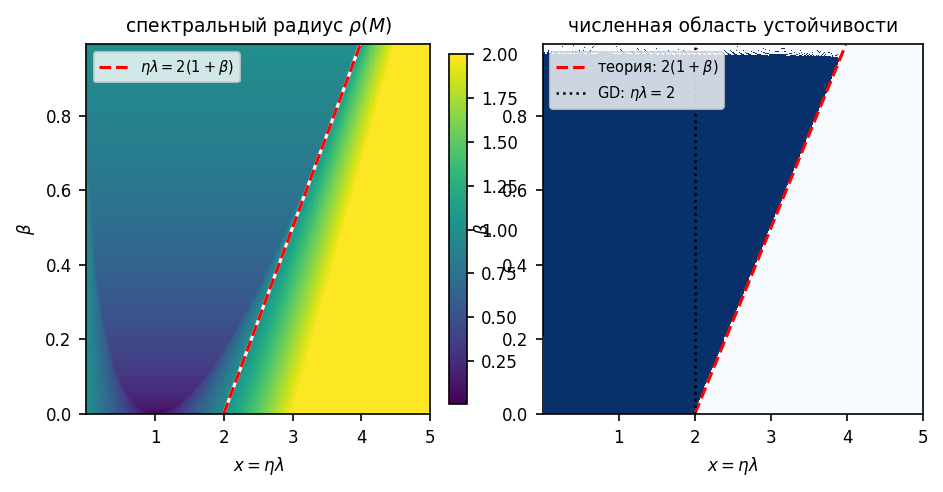
\includegraphics[width=\linewidth]{f05_theory_stability.png}
  \caption{Область устойчивости метода тяжёлого шарика на квадратичной функции.
  Слева --- спектральный радиус матрицы перехода (значения обрезаны сверху
  на уровне 2); белая линия --- уровень $\rho=1$, красная штриховая ---
  аналитическая граница $\eta\lambda = 2(1+\beta)$. Справа --- численно
  определённая область устойчивости.}
  \label{fig:theory}
\end{figure}

\subsection{Почему в нелинейном случае граница усложняется}

Предложение~\ref{prop:stab} даёт гладкую границу: в плоскости $(x,\beta)$ это
прямая. Однако три обстоятельства разрушают эту гладкость при переходе к
нейронной сети.

Во-первых, в многомерном случае $L$ имеет спектр кривизн
$\lambda_1,\dots,\lambda_d$, и условие устойчивости должно выполняться
одновременно для всех мод: $\eta\lambda_i < 2(1+\beta)$. Граница области
устойчивости определяется максимальным собственным значением гессиана, которое
само зависит от точки в пространстве параметров, а значит --- от всей
предыстории траектории.

Во-вторых, при обучении нейронной сети гессиан не постоянен: система, вышедшая
за порог устойчивости по одной моде, не обязана расходиться, поскольку может
перейти в область меньшей кривизны (catapult-механизм~\cite{lewkowycz2020}) и
стабилизироваться на грани устойчивости~\cite{cohen2021}. Итоговый исход
зависит от того, успеет ли траектория попасть в такую область раньше, чем
норма весов достигнет переполнения; это делает исход чувствительным к сколь
угодно малым изменениям гиперпараметров.

В-третьих, при потере устойчивости неподвижной точки нелинейная система не
уходит на бесконечность сразу, а проходит через каскад удвоения
периода~\cite{feigenbaum1978} и хаос. На рис.~\ref{fig:bif} показана
бифуркационная диаграмма для скалярной нелинейной задачи
$L(w) = \tfrac12 (w^2-y)^2$ при трёх значениях инерции. Видно, что рост
$\beta$ смещает каскад бифуркаций в область меньших $\eta$ и делает переход
более резким: при $\beta=0.9$ окно устойчивого поведения по $\eta$ существенно
сужается, хотя для квадратичной модели инерция допустимый шаг, наоборот,
расширяет. Это принципиальное различие между линейным и нелинейным случаем и
объясняет, почему граница, гладкая в теории для квадратики, становится
изрезанной для сети.

\begin{figure}[htbp]
  \centering
  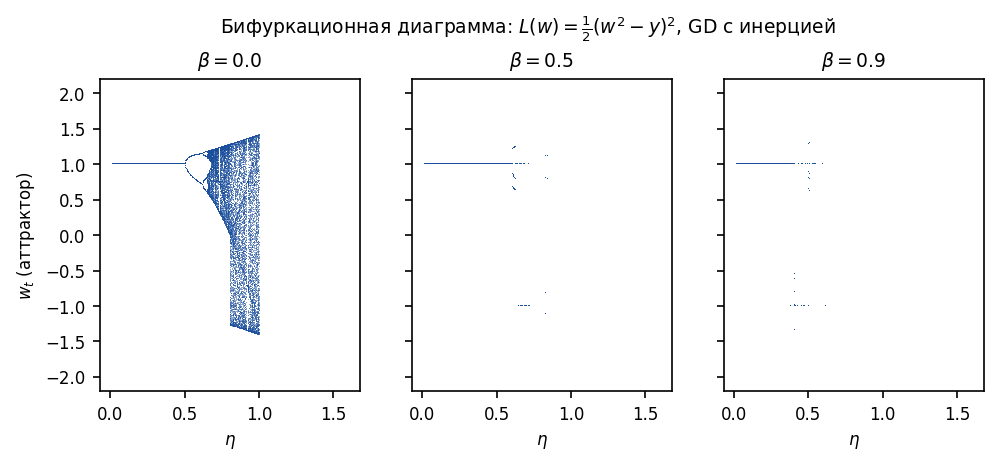
\includegraphics[width=\linewidth]{f06_bifurcation.png}
  \caption{Бифуркационная диаграмма для нелинейной скалярной задачи
  $L(w)=\tfrac12(w^2-y)^2$ при $y=1$: показаны последние 120 из 600 итераций
  для каждого $\eta$. Слева направо: $\beta=0$, $\beta=0.5$, $\beta=0.9$.}
  \label{fig:bif}
\end{figure}

\section{Объект и методы исследования}\label{sec:methods}

\subsection{Вычислительная схема: ансамблевая векторизация}

Прямолинейная реализация сканирования требует обучить $n^2$ сетей независимо;
при $n=512$ и $T=400$ это $10^8$ итераций и, в наивном цикле, десятки часов
машинного времени. В настоящей работе используется другая схема: все узлы
сетки обучаются \emph{одновременно} как ансамбль независимых сетей.

Веса хранятся в тензорах формы $(G, h, d_{in})$ и $(G, d_{out}, h)$, где
$G$ --- число конфигураций в текущем блоке, а гиперпараметры --- в векторах
формы $(G,)$, транслируемых по осям весов. Прямой и обратный проход
записываются через пакетные свёртки индексов:
\begin{center}
\ttfamily\small
H = einsum('nd,ghd->gnh', X, W0);\quad
gW0 = einsum('gnh,nd->ghd', gh, X)
\end{center}
и так далее. Это сводит всю итерацию к нескольким вызовам BLAS и даёт
ускорение примерно на два порядка по сравнению с поэлементным циклом.
Расчёт ведётся блоками по $4096$ конфигураций, что ограничивает пик потребления
памяти примерно $200$~МБ.

Градиенты вычисляются вручную (без автоматического дифференцирования), что
обеспечивает полный контроль над порядком операций и, следовательно, побитовую
воспроизводимость. Конфигурации, достигшие переполнения, не исключаются из
расчёта, но их градиенты обнуляются через \texttt{nan\_to\_num}, чтобы
переполнение в одной конфигурации не портило соседние через общие
арифметические операции; факт переполнения при этом запоминается и определяет
режим NaN/Inf.

\subsection{Протокол экспериментов}

Общие параметры, если не указано иное: $d_{in}=d_{out}=h=16$; инициализация
весов нормальным распределением с масштабом $1.0$, одна и та же для всех узлов
сетки; число итераций $T=400$; тип данных \texttt{float64}; разрешение сетки
$256\times256$, для двух опорных карт --- $512\times512$.

Базовый набор данных --- одна обучающая пара ($|\mathcal{D}|=1$) со случайными
$x$ и $y$ из стандартного нормального распределения. Этот выбор унаследован от
работы~\cite{sohl2024}, где случай $|\mathcal{D}|=1$ рассматривается как
минимальный, в котором явление уже наблюдается, и не осложнён усреднением по
выборке. Для экспериментов с мини-батчами и со структурированными данными
используются наборы из 32 и 16 примеров соответственно.

Набор \texttt{sklearn digits} преобразуется следующим образом: изображения
$8\times8$ разворачиваются в векторы длины 64, центрируются, проецируются на
первые 16 главных компонент всей выборки и нормируются на единичное
стандартное отклонение; целевые векторы --- one-hot представление класса в
$\{-1,+1\}^{16}$. Такое преобразование позволяет использовать ту же
архитектуру, что и для случайных данных, и делает сравнение корректным.

\subsection{Выбор окон сканирования}

Порог устойчивости зависит от кривизны функции потерь, а та --- от активации,
объёма данных и оптимизатора. Поэтому единое окно по $\eta$ для всех
конфигураций непригодно: например, для ReLU при $|\mathcal{D}|=1$ во всём
диапазоне $\eta\in[10^{-2},10]$ доля сходимости составляет $0.99$, то есть
граница просто не попадает в окно. Окна подбирались так, чтобы граница
находилась внутри области сканирования, а доли режимов были нетривиальны.
Конкретные диапазоны указаны при каждом эксперименте; следствия этого выбора
для сопоставимости оценок обсуждаются в разделе~\ref{sec:limitations}.

\subsection{Последовательность зумов}

Центр зума выбирается автоматически, а не вручную: по опорной карте
$(\eta,\beta)$ вычисляется бинарная граница, к ней применяется усредняющий
фильтр $41\times41$, и центром объявляется точка максимума плотности границы,
удалённая не менее чем на 64 пикселя от краёв. Для базовой карты это дало
точку $\eta^\ast \approx 0.369$, $\beta^\ast \approx 0.300$. На уровне $k$
окно сжимается вдвое по $\log_{10}\eta$ и по $\beta$ относительно центра.

\subsection{Программная среда и ресурсы}

Реализация выполнена на Python 3.12 с использованием NumPy (линейная алгебра),
SciPy (морфологические операции), scikit-image (скелетонизация),
scikit-learn (набор digits) и Matplotlib (визуализация). PyTorch не
использовался: в целевой вычислительной среде он недоступен, а ансамблевая
векторизация на NumPy оказалась достаточной по производительности.
Вычисления проводились на одном ядре CPU; суммарное машинное время всех
экспериментов, вошедших в отчёт, составило \TotalHours~ч.

Воспроизводимость обеспечивается фиксацией: seed генератора случайных чисел
($42$ для данных, $42+1000$ для инициализации весов, $42+7$ для порядка
примеров в мини-батчах), типа точности, разрешения сетки, числа итераций и
порогов классификации режимов. Все параметры каждого запуска сохраняются в
JSON рядом с результатом, а числа в таблицах и в тексте настоящего отчёта
подставляются автоматически из этих файлов, что исключает расхождение между
текстом и данными.

\section{Результаты экспериментов}\label{sec:results}

\subsection{Репликация базового эксперимента}

На рис.~\ref{fig:base} представлена карта обучаемости для базовой конфигурации
(tanh, $|\mathcal{D}|=1$, полный батч, разрешение $512\times512$). Слева ---
карта четырёх режимов, справа --- непрерывная сине-красная карта в стиле
предыдущей НИР, где насыщенность синего пропорциональна сумме нормализованных
loss по итерациям, а красного --- обратной величине.

\begin{figure}[htbp]
  \centering
  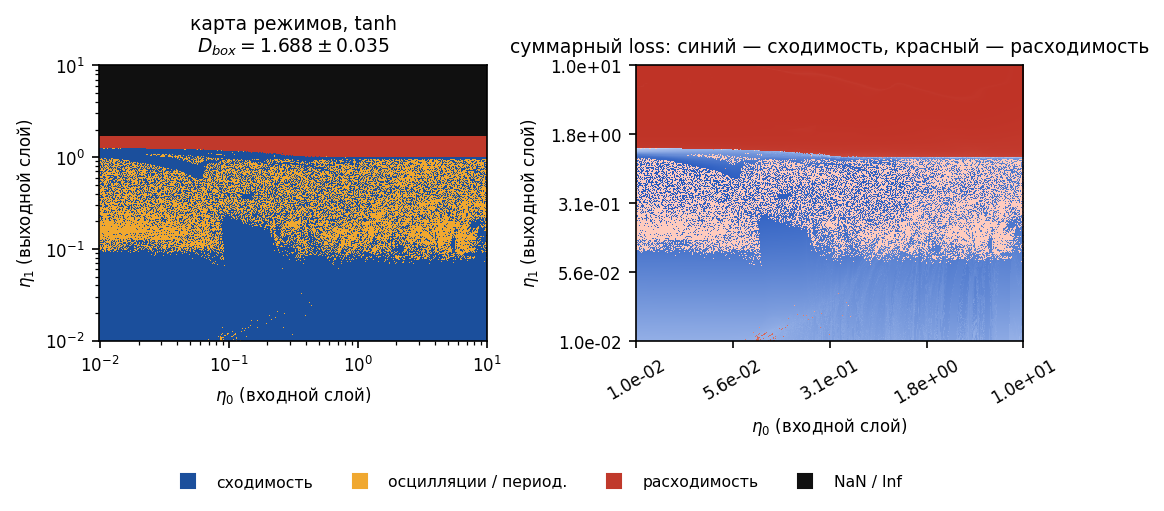
\includegraphics[width=\linewidth]{f01_base_tanh.png}
  \caption{Базовая карта обучаемости в плоскости $(\eta_0,\eta_1)$, активация
  tanh, разрешение $512\times512$, $T=400$ итераций.}
  \label{fig:base}
\end{figure}

Качественная картина воспроизводит результат предыдущей НИР: существуют
протяжённые связные области успешного обучения, граница между ними и областью
расходимости не является гладкой кривой, а оптимальные по скорости
конфигурации располагаются вблизи границы. Существенное отличие от предыдущей
работы состоит в том, что значительную часть карты занимает режим ограниченных
незатухающих колебаний (доля \DBaseTanhConv{} приходится на сходимость), который
при бинарном критерии предыдущей НИР был бы отнесён к сходимости.

Измеренная размерность границы составила
$D_{\mathrm{box}} = \DBaseTanh \pm \DBaseTanhS$.

Сравнение активаций осложняется тем, что порог устойчивости у них различен
(см.~табл.~\ref{tab:act}). В общем окне $\eta\in[10^{-2},10]$ для ReLU при
$|\mathcal{D}|=1$ доля сходимости равна $0.99$, а для линейной сети, наоборот,
$0.07$: граница выходит за пределы окна. Поэтому дополнительно выполнены
прогоны в окнах, центрированных на собственном пороге каждой конфигурации, и
прогоны на общем наборе из 32 примеров, где сравнение активаций корректно:
tanh даёт $\DTanhMb$, ReLU --- $\DReluMbLow$.

\begin{table}[htbp]
  \centering
  \caption{Размерность границы для разных активаций и окон сканирования.
  Столбцы «сход.», «осц.», «расх.», «NaN» --- доли соответствующих режимов.}
  \label{tab:act}
  \small
  \begin{tabular}{llccccc}
\toprule
Активация & Окно по $\eta$ & $D_{\mathrm{box}}$ & сход. & осц. & расх. & NaN\\
\midrule
tanh & $[10^{-2},10]$, $|\mathcal{D}|=1$, $512^2$ & $1.688 \pm 0.035$ & 0.49 & 0.19 & 0.06 & 0.26\\
ReLU & $[10^{-2},10]$, $|\mathcal{D}|=1$ & $1.160 \pm 0.008$ & 0.99 & 0.01 & 0.00 & 0.00\\
линейная & $[10^{-2},10]$, $|\mathcal{D}|=1$ & $1.512 \pm 0.067$ & 0.07 & 0.02 & 0.00 & 0.91\\
линейная & $[10^{-4},10^{-1}]$, $|\mathcal{D}|=1$ & $1.565 \pm 0.033$ & 0.75 & 0.15 & 0.00 & 0.10\\
tanh & $[10^{-1},10^{3}]$, $|\mathcal{D}|=32$ & $1.433 \pm 0.050$ & 0.38 & 0.07 & 0.02 & 0.54\\
ReLU & $[10^{-3},10]$, $|\mathcal{D}|=32$ & $1.282 \pm 0.045$ & 0.47 & 0.11 & 0.00 & 0.43\\
ReLU & $[10^{-1},10^{3}]$, $|\mathcal{D}|=32$ & $1.074 \pm 0.010$ & 0.06 & 0.00 & 0.00 & 0.94\\
\bottomrule
\end{tabular}

\end{table}

Рис.~\ref{fig:act} показывает карты для трёх активаций в общем окне; хорошо
видно, что для ReLU граница в это окно не попадает.

\begin{figure}[htbp]
  \centering
  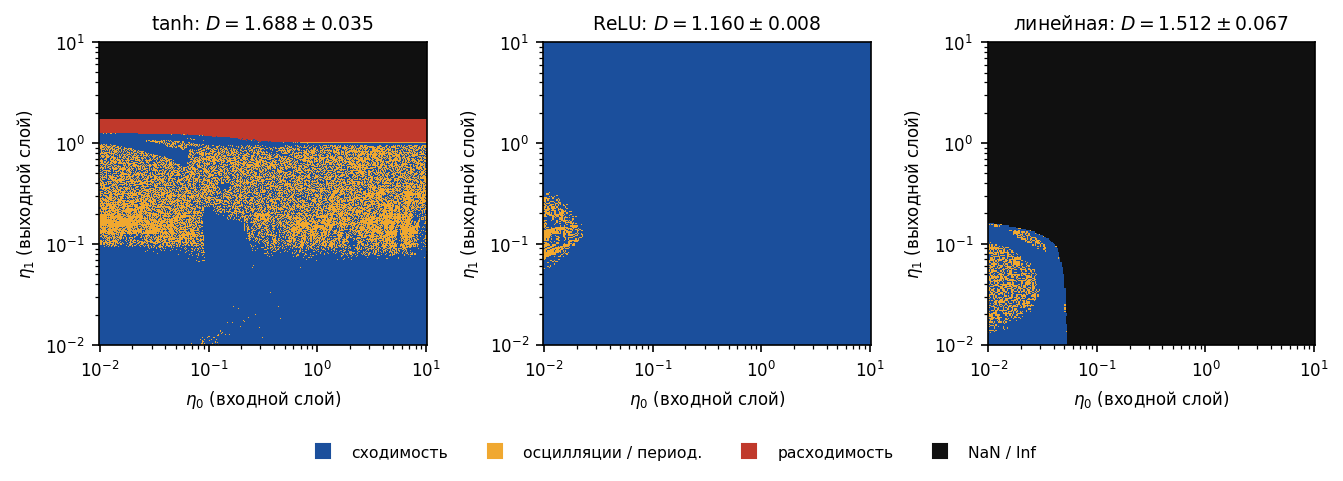
\includegraphics[width=\linewidth]{f02_activations.png}
  \caption{Карты режимов для активаций tanh, ReLU и линейной в общем окне
  $\eta\in[10^{-2},10]$.}
  \label{fig:act}
\end{figure}

Линейность зависимости $\log N(\varepsilon)$ от $\log\varepsilon$,
подтверждающая применимость оценки~\eqref{eq:box}, показана на
рис.~\ref{fig:boxcount}.

\begin{figure}[htbp]
  \centering
  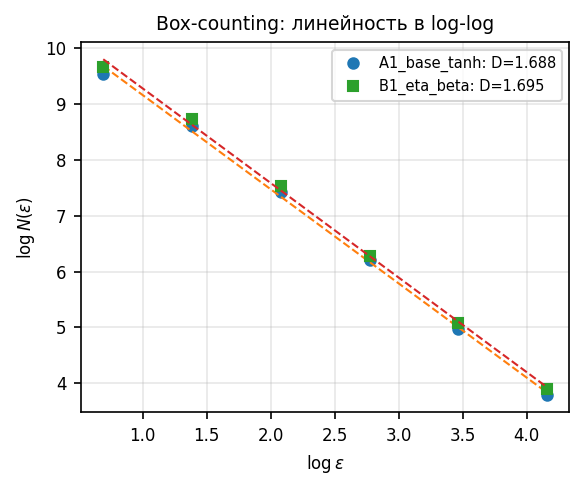
\includegraphics[width=0.62\linewidth]{f03_boxcounting.png}
  \caption{Box-counting: зависимость числа непустых ячеек от размера ячейки
  в логарифмических координатах для базовой карты и для сечения
  $(\eta,\beta)$.}
  \label{fig:boxcount}
\end{figure}

\subsection{Сечение $(\eta,\beta)$: инерция}

Центральный результат работы представлен на рис.~\ref{fig:etabeta}: сечение
пространства гиперпараметров по шагу обучения и коэффициенту инерции при
общем для обоих слоёв $\eta$.

\begin{figure}[htbp]
  \centering
  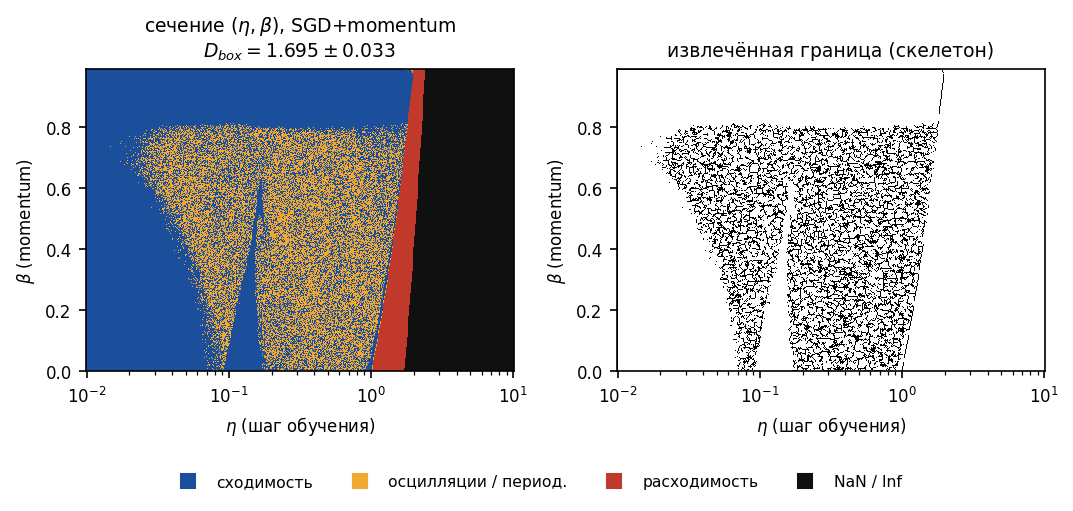
\includegraphics[width=\linewidth]{f04_eta_beta.png}
  \caption{Сечение $(\eta,\beta)$ для SGD с инерцией, разрешение
  $512\times512$. Справа --- извлечённая скелетонизированная граница
  множества сходимости.}
  \label{fig:etabeta}
\end{figure}

Измеренная размерность $D_{\mathrm{box}} = \DEtaBeta \pm \DEtaBetaS$ совпадает
в пределах погрешности с размерностью базовой карты $(\eta_0,\eta_1)$,
равной $\DBaseTanh \pm \DBaseTanhS$. Таким образом, добавление инерции не
делает границу обучаемости гладкой: первая из проверяемых гипотез
подтверждается.

Структура карты согласуется с теорией раздела~\ref{sec:theory}. При малых
$\eta$ обучение сходится при любом $\beta$; при росте $\eta$ система сначала
входит в область ограниченных колебаний, и лишь затем --- в область
переполнения. Граница области сходимости смещается влево с ростом $\beta$,
что отражает увеличение эффективного шага: в стационарном режиме накопленная
скорость в схеме~\eqref{eq:hb} превышает мгновенный градиент в $1/(1-\beta)$
раз. При $\beta\gtrsim0.8$ область незатухающих колебаний практически исчезает,
уступая место резкому переходу от сходимости к переполнению.

\subsection{Затухание весов и размер батча}

Результаты для сечения $(\eta,\lambda_{wd})$ и для мини-батчей сведены в
табл.~\ref{tab:sections} и~\ref{tab:mb}, карты приведены на
рис.~\ref{fig:wd}--\ref{fig:mb}.

\begin{table}[htbp]
  \centering
  \caption{Размерность границы в основных сечениях (разрешение $256\times256$,
  кроме отмеченных отдельно).}
  \label{tab:sections}
  \small
  \input{tables/tab_sections.tex}
\end{table}

\begin{figure}[htbp]
  \centering
  \begin{subfigure}{0.46\linewidth}
    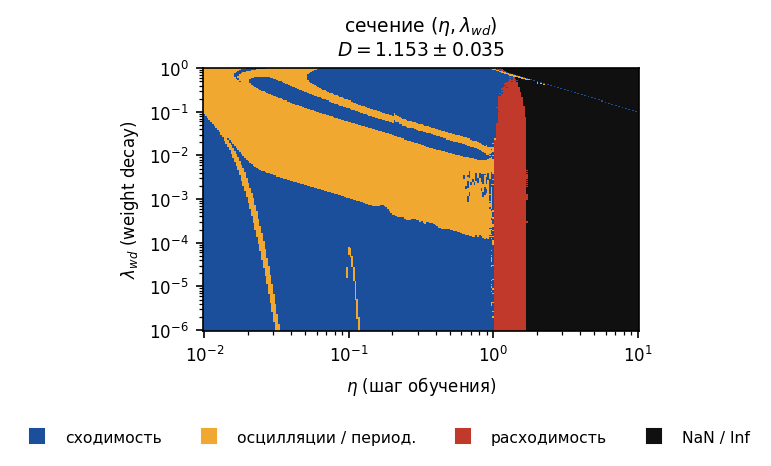
\includegraphics[width=\linewidth]{f07_eta_wd.png}
    \caption{сечение $(\eta,\lambda_{wd})$}
  \end{subfigure}\hfill
  \begin{subfigure}{0.52\linewidth}
    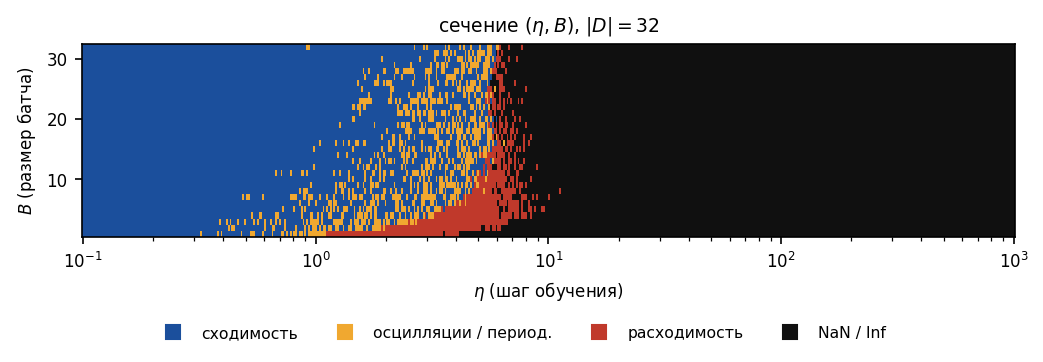
\includegraphics[width=\linewidth]{f08_eta_batch.png}
    \caption{сечение $(\eta,B)$}
  \end{subfigure}
  \caption{Влияние затухания весов и размера батча.}
  \label{fig:wd}
\end{figure}

Затухание весов заметно сглаживает границу: $D_{\mathrm{box}} = \DEtaWd \pm \DEtaWdS$
против $\DSgd \pm \DSgdS$ для карты $(\eta_0,\eta_1)$ при том же разрешении.
Механизм прозрачен: слагаемое $\lambda_{wd}W$ добавляет к гессиану
изотропный сдвиг $\lambda_{wd}I$, что при больших $\lambda_{wd}$ подавляет
различие между направлениями разной кривизны и делает порог устойчивости
почти не зависящим от точки в пространстве параметров.

Для сечения $(\eta,B)$ карта режимов построена (рис.~\ref{fig:wd}б), однако
размерность по нему не оценивалась: полоса $512\times32$ не даёт достаточного
числа масштабов $\varepsilon$ для устойчивой регрессии~\eqref{eq:box}, и
результат оказывается неопределённым. Вместо этого влияние размера батча
измерено по полноценным картам $(\eta_0,\eta_1)$ при фиксированных $B$.

\begin{table}[htbp]
  \centering
  \caption{Влияние размера мини-батча ($|\mathcal{D}|=32$, tanh).}
  \label{tab:mb}
  \small
  \begin{tabular}{lccccc}
\toprule
Конфигурация & $D_{\mathrm{box}}$ & сход. & осц. & расх. & NaN\\
\midrule
$B=1$ & $1.722 \pm 0.074$ & 0.17 & 0.09 & 0.13 & 0.61\\
$B=4$ & $1.568 \pm 0.050$ & 0.30 & 0.08 & 0.09 & 0.53\\
$B=32$ (полный батч) & $1.433 \pm 0.050$ & 0.38 & 0.07 & 0.02 & 0.54\\
\bottomrule
\end{tabular}

\end{table}

\begin{figure}[htbp]
  \centering
  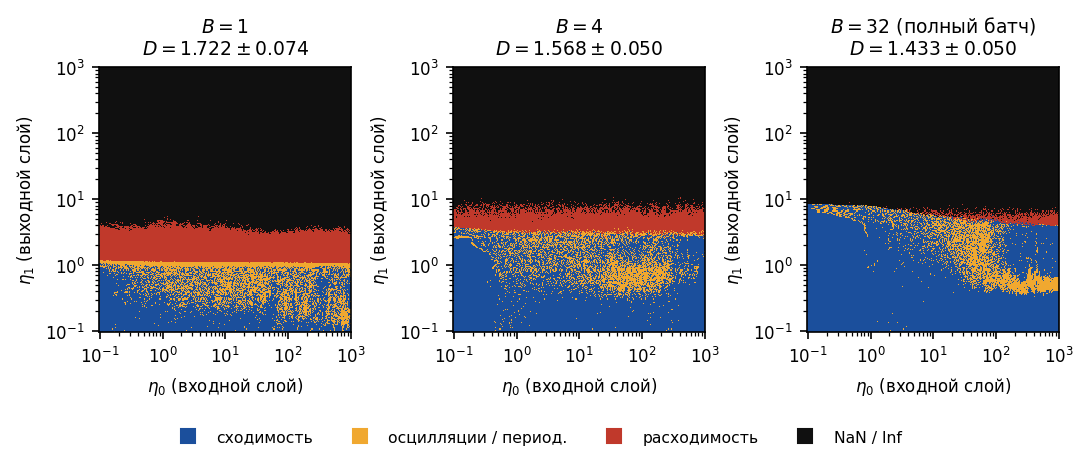
\includegraphics[width=\linewidth]{f09_minibatch.png}
  \caption{Карты обучаемости при разных размерах мини-батча.}
  \label{fig:mb}
\end{figure}

Наблюдается монотонный тренд: $B=1$ даёт $\DMbOne$, $B=4$ --- $\DMbFour$,
полный батч $B=32$ --- $\DMbFull$. Уменьшение батча увеличивает изрезанность
границы. Это согласуется с интерпретацией~\cite{kong2020}: стохастичность
выборки играет роль дополнительного мелкомасштабного возмущения целевой
функции, а по результатам~\cite{liu2024} именно мелкомасштабная невыпуклость
и порождает фрактальную границу. Вторая гипотеза, таким образом,
подтверждается для размера батча, но в части затухания весов --- лишь при
достаточно больших $\lambda_{wd}$ (см.~ниже раздел~\ref{sec:3d}).

\subsection{Сравнение оптимизаторов}

Результаты сравнения четырёх методов приведены в табл.~\ref{tab:opt} и на
рис.~\ref{fig:opt}.

\begin{table}[htbp]
  \centering
  \caption{Сравнение оптимизаторов и сечений Adam (разрешение $256\times256$).}
  \label{tab:opt}
  \small
  \begin{tabular}{lccccc}
\toprule
Конфигурация & $D_{\mathrm{box}}$ & сход. & осц. & расх. & NaN\\
\midrule
SGD & $1.633 \pm 0.041$ & 0.49 & 0.19 & 0.06 & 0.26\\
SGD+momentum ($\beta=0.9$) & $1.037 \pm 0.011$ & 0.82 & 0.00 & 0.02 & 0.16\\
Adam & $1.322 \pm 0.054$ & 0.82 & 0.05 & 0.14 & 0.00\\
RMSprop & $1.508 \pm 0.068$ & 0.20 & 0.54 & 0.26 & 0.00\\
Adam, сечение $(\eta,\beta_1)$ & $1.698 \pm 0.071$ & 0.48 & 0.52 & 0.00 & 0.00\\
Adam, сечение $(\eta,\beta_2)$ & $1.727 \pm 0.073$ & 0.28 & 0.72 & 0.00 & 0.00\\
\bottomrule
\end{tabular}

\end{table}

\begin{figure}[htbp]
  \centering
  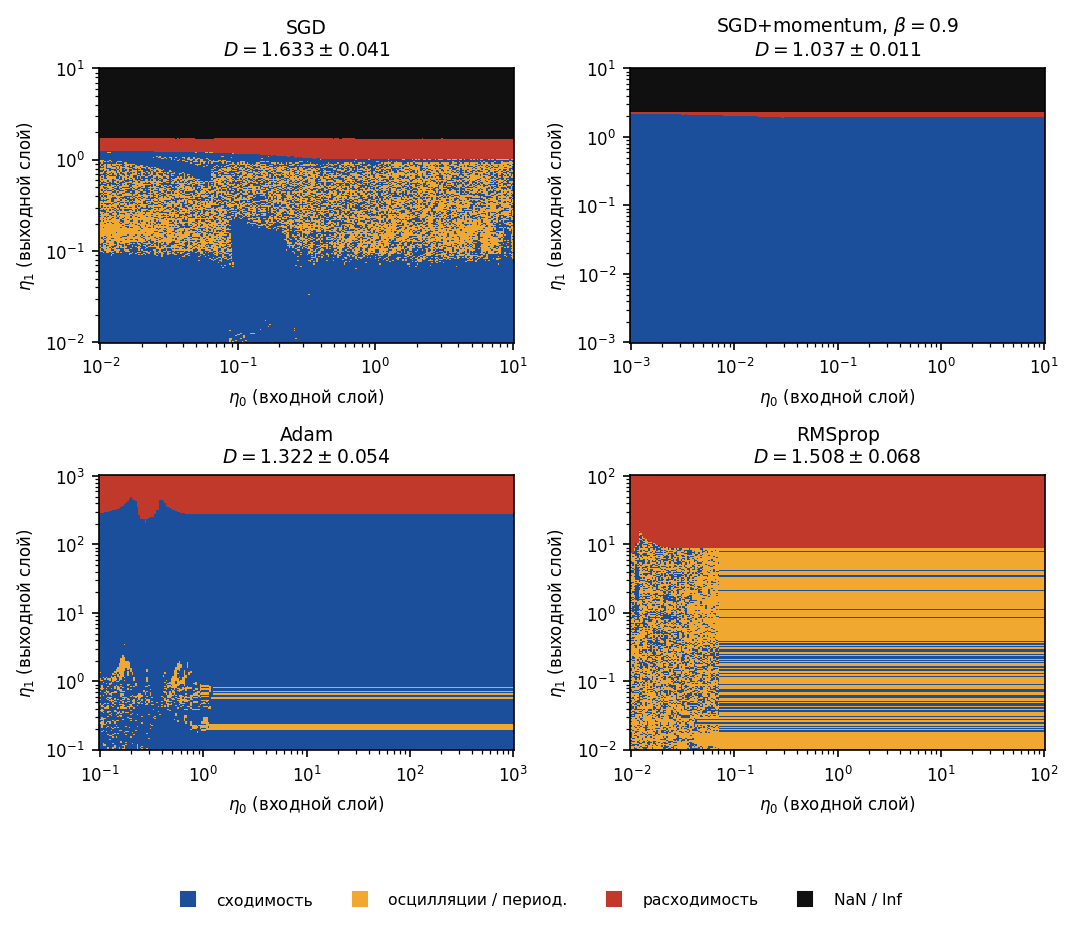
\includegraphics[width=\linewidth]{f10_optimizers.png}
  \caption{Карты обучаемости в плоскости $(\eta_0,\eta_1)$ для четырёх
  оптимизаторов. Диапазоны по осям различны и подобраны под собственный порог
  каждого метода.}
  \label{fig:opt}
\end{figure}

В плоскости $(\eta_0,\eta_1)$ Adam действительно даёт более гладкую границу,
чем SGD: $\DAdam$ против $\DSgd$. Однако наименьшую размерность даёт вовсе не
адаптивный метод, а SGD с фиксированной инерцией $\beta=0.9$: $\DMomentum$.
RMSprop занимает промежуточное положение ($\DRmsprop$).

Более того, если сечь пространство гиперпараметров вдоль осей самого Adam,
картина меняется на противоположную (рис.~\ref{fig:adamsec}): сечение
$(\eta,\beta_1)$ даёт $\DAdamBOne$, а $(\eta,\beta_2)$ --- $\DAdamBTwo$, то
есть выше, чем у SGD в базовом сечении. Гипотеза о сглаживающем действии
адаптивных методов, таким образом, подтверждается лишь частично и требует
переформулировки, к чему мы вернёмся в разделе~\ref{sec:discussion}.

\begin{figure}[htbp]
  \centering
  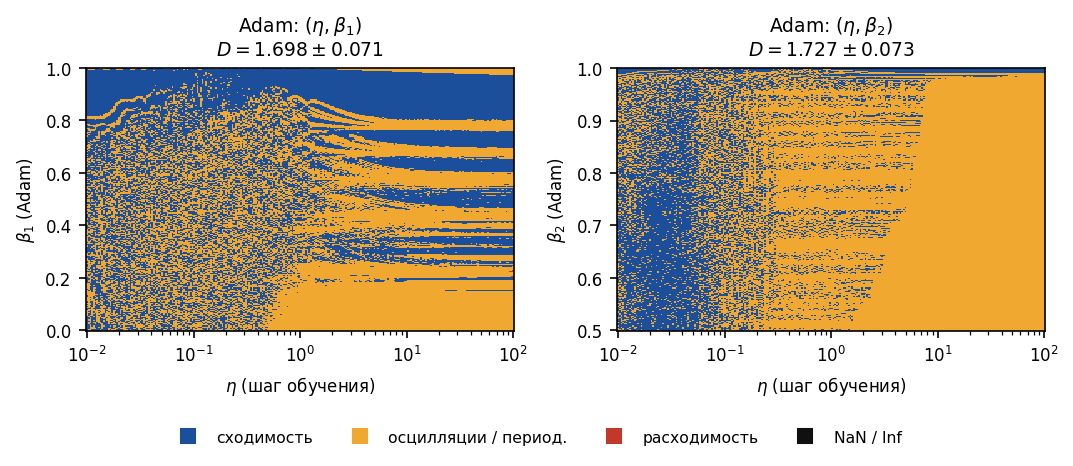
\includegraphics[width=\linewidth]{f11_adam_sections.png}
  \caption{Сечения пространства гиперпараметров Adam по $\beta_1$ и $\beta_2$.}
  \label{fig:adamsec}
\end{figure}

Отдельного внимания заслуживает структура карт Adam и RMSprop: на них хорошо
видны горизонтальные полосы, почти не зависящие от $\eta_0$. Это прямое
следствие покоординатной нормализации: величина шага по каждому весу равна
приблизительно $\eta$ независимо от масштаба градиента, поэтому динамика
разделяется по слоям, и карта становится почти сепарабельной. Именно эта
сепарабельность, а не подавление хаоса как такового, и снижает измеряемую
размерность границы в плоскости $(\eta_0,\eta_1)$.

\subsection{Случайные и структурированные данные}

\begin{table}[htbp]
  \centering
  \caption{Влияние структуры данных ($|\mathcal{D}|=16$, полный батч, tanh).}
  \label{tab:data}
  \small
  \begin{tabular}{lccccc}
\toprule
Конфигурация & $D_{\mathrm{box}}$ & сход. & осц. & расх. & NaN\\
\midrule
случайные данные, $|D|=16$ & $1.284 \pm 0.070$ & 0.39 & 0.02 & 0.02 & 0.57\\
digits (PCA-16), $|D|=16$ & $1.494 \pm 0.073$ & 0.34 & 0.04 & 0.02 & 0.60\\
\bottomrule
\end{tabular}

\end{table}

\begin{figure}[htbp]
  \centering
  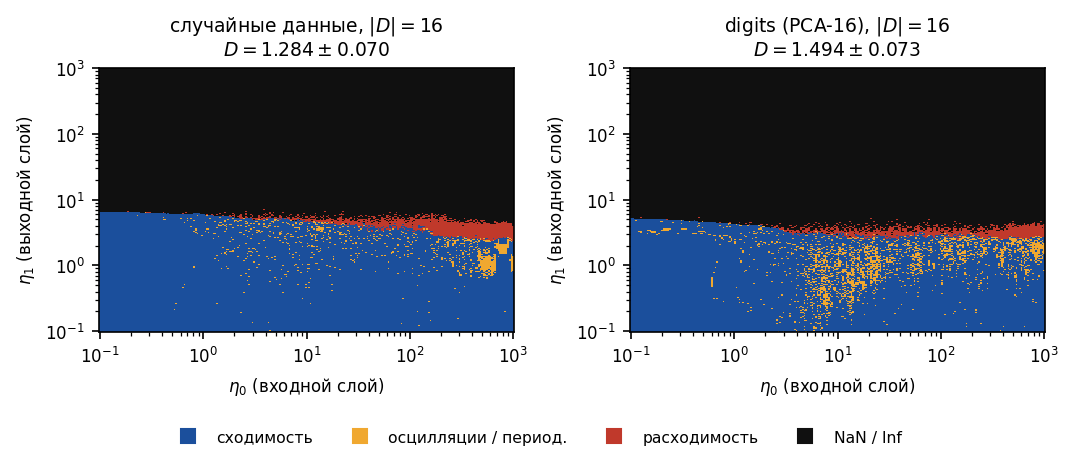
\includegraphics[width=\linewidth]{f12_data.png}
  \caption{Границы обучаемости на случайных данных и на наборе digits.}
  \label{fig:data}
\end{figure}

При переходе от случайных данных к структурированным размерность возрастает:
$\DSynth$ против $\DDigits$ (табл.~\ref{tab:data}, рис.~\ref{fig:data}).
Правдоподобное объяснение состоит в том, что у случайных данных спектр
ковариационной матрицы входов близок к вырожденному по масштабу (все
собственные значения одного порядка), тогда как у digits после проекции на
главные компоненты спектр существенно неоднороден. Многомасштабность целевой
функции --- именно тот фактор, который по результатам~\cite{kong2020}
порождает хаотическое поведение детерминированного градиентного спуска.
Фрактальность границы, таким образом, не является артефактом синтетических
данных.

\subsection{Трёхмерное пространство $(\eta,\beta,\lambda_{wd})$}\label{sec:3d}

Трёхмерный эксперимент реализован как набор двумерных сечений
$(\eta,\beta)$ при четырёх значениях затухания весов
(табл.~\ref{tab:wd}, рис.~\ref{fig:wdslices}).

\begin{table}[htbp]
  \centering
  \caption{Сечения трёхмерного пространства $(\eta,\beta,\lambda_{wd})$.}
  \label{tab:wd}
  \small
  \input{tables/tab_wd_slices.tex}
\end{table}

\begin{figure}[htbp]
  \centering
  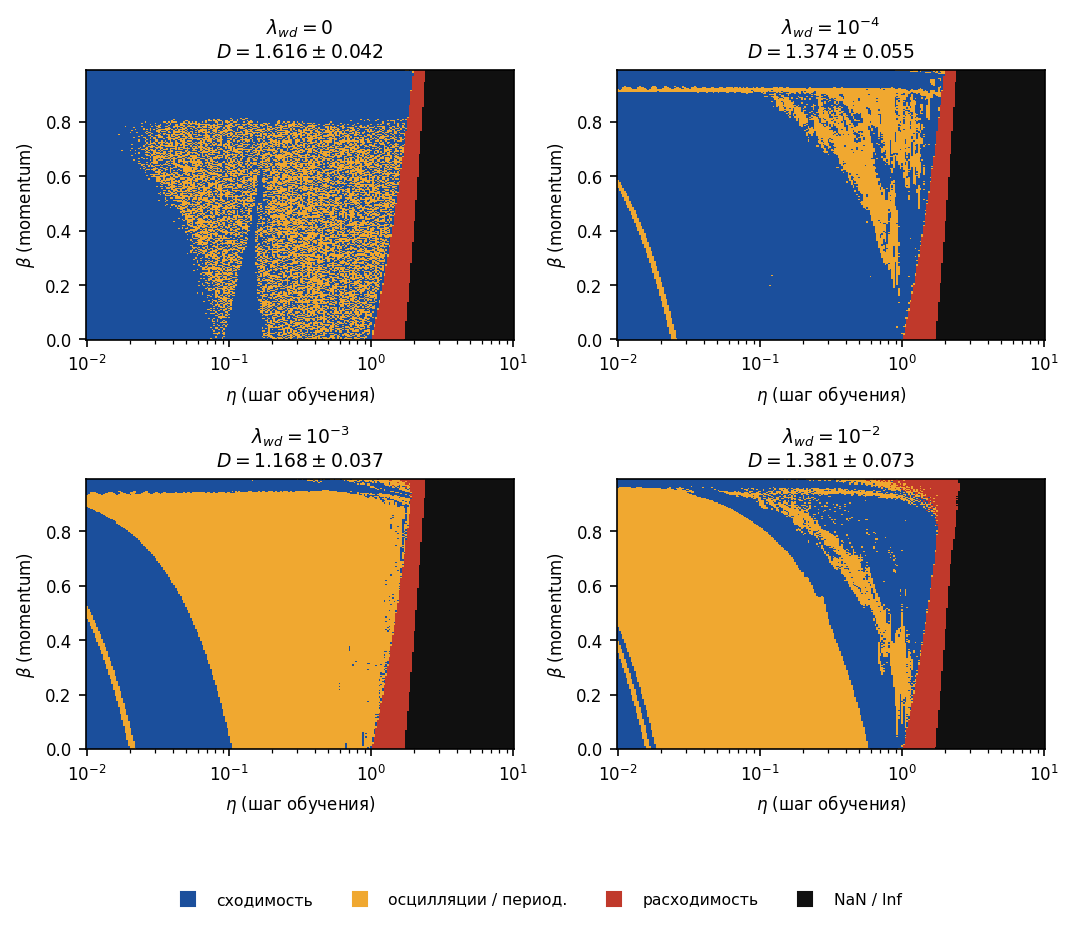
\includegraphics[width=\linewidth]{f13_wd_slices.png}
  \caption{Сечения $(\eta,\beta)$ при разных значениях $\lambda_{wd}$.}
  \label{fig:wdslices}
\end{figure}

Зависимость немонотонна: $\lambda_{wd}=0$ даёт $\DWdZero$, $10^{-4}$ ---
$\DWdOne$, $10^{-3}$ --- $\DWdTwo$, но $10^{-2}$ --- снова $\DWdThree$.
Содержательно это означает, что умеренная регуляризация сглаживает границу,
а при дальнейшем росте $\lambda_{wd}$ появляется новый эффект: затухание весов
начинает конкурировать с обучением, и возникает дополнительная граница между
режимом обучения и режимом стягивания весов к нулю, которая сама по себе
нерегулярна. Заметно также, что доля осцилляционного режима резко возрастает
(с $0.20$ до $0.48$).

Отсюда следует прямой ответ на вопрос, поставленный в задании: по набору
двумерных сечений судить о сложности границы в полном трёхмерном пространстве
можно лишь с осторожностью. Немонотонность $D(\lambda_{wd})$ показывает, что
сечения не являются «типичными» срезами однородного объекта; каждое сечение
характеризует локальную геометрию границы вблизи выбранной плоскости, а не
глобальную структуру. Строгое утверждение о размерности трёхмерной границы
потребовало бы прямого box-counting в трёхмерной сетке, что превышает
доступные вычислительные ресурсы: сетка $256^3$ при $T=400$ потребовала бы
примерно в 256 раз больше времени, чем одно двумерное сканирование.

\subsection{Последовательность зумов}

Пять уровней зума вокруг автоматически выбранной точки границы
($\eta^\ast\approx0.369$, $\beta^\ast\approx0.300$) показаны на
рис.~\ref{fig:zoom}, измеренные размерности --- в табл.~\ref{tab:zoom}.

\begin{table}[htbp]
  \centering
  \caption{Размерность границы на разных уровнях зума в плоскости
  $(\eta,\beta)$.}
  \label{tab:zoom}
  \small
  \input{tables/tab_zoom.tex}
\end{table}

\begin{figure}[htbp]
  \centering
  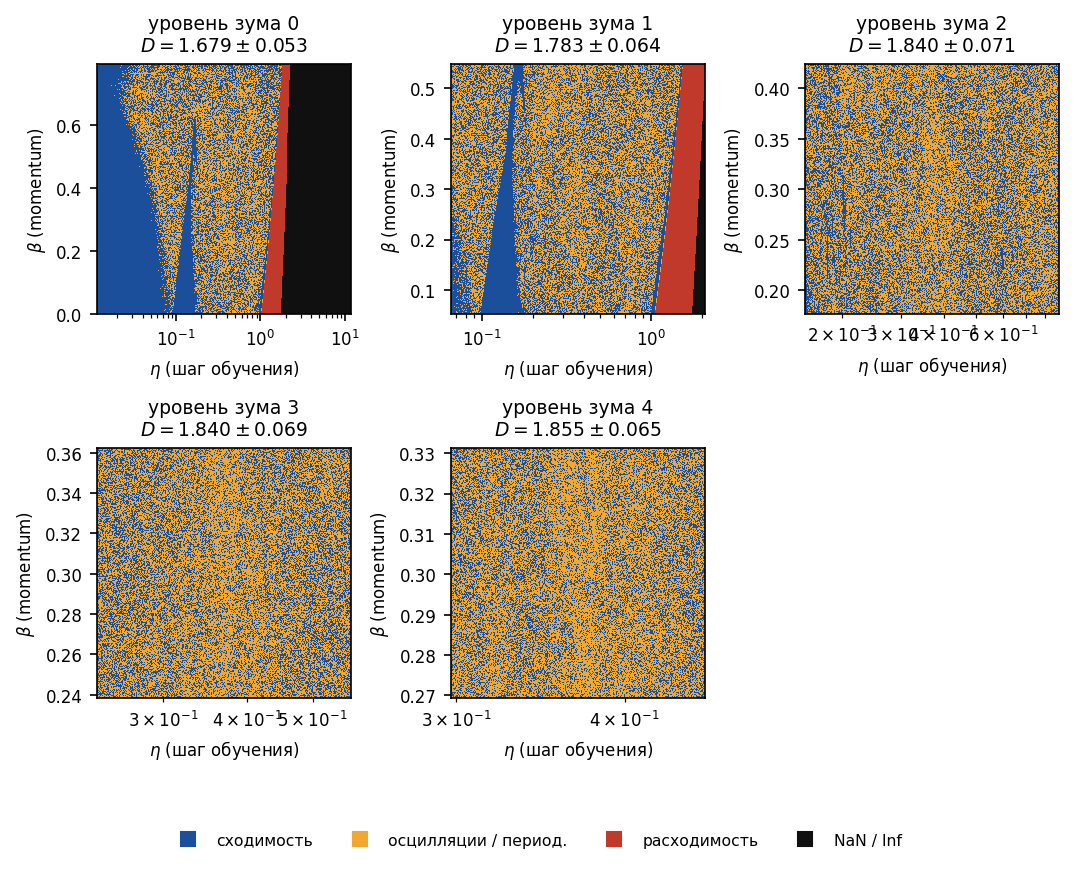
\includegraphics[width=\linewidth]{f14_zoom.png}
  \caption{Последовательность зумов: каждый следующий уровень сужает окно
  вдвое по $\log\eta$ и по $\beta$.}
  \label{fig:zoom}
\end{figure}

Структура сохраняется на всех пяти уровнях: качественный характер картины не
меняется, что и означает самоподобие. Однако, в отличие от предыдущей НИР, где
размерность по уровням зума была практически постоянной
($\sigma = 0.009$), здесь наблюдается систематический рост от
$1.679$ на нулевом уровне до $1.855$ на четвёртом с последующим насыщением;
медиана составляет $\DZoomMedian$ при стандартном отклонении $\DZoomStd$.

Причина роста видна из долей режимов: с углублением зума область переполнения
исчезает полностью, а доля осцилляционного режима возрастает с $0.26$ до
$0.63$. Иными словами, при увеличении мы попадаем внутрь зоны, где режимы
сходимости и колебаний перемешаны на масштабе отдельных узлов сетки, и
измеряемое множество перестаёт быть кривой, приближаясь к площадному
заполнению ($D\to2$). Это не столько свойство границы, сколько указание на
предел применимости самой процедуры: box-counting по бинаризованной карте
измеряет геометрию перемешанной зоны, а не гладкой кривой. Рис.~\ref{fig:selfsim}
показывает извлечённые границы на нулевом и четвёртом уровнях.

\begin{figure}[htbp]
  \centering
  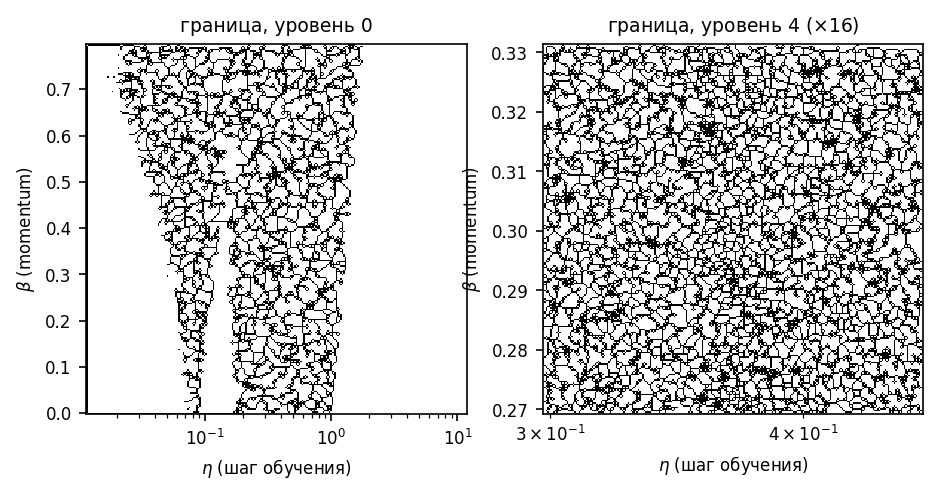
\includegraphics[width=\linewidth]{f16_boundary_selfsim.png}
  \caption{Извлечённая граница на нулевом и четвёртом уровнях зума.}
  \label{fig:selfsim}
\end{figure}

\subsection{Влияние численной точности}

Сравнение расчёта в \texttt{float64} и \texttt{float32} для одного и того же
сечения $(\eta,\beta)$ приведено в табл.~\ref{tab:prec} и на
рис.~\ref{fig:prec}.

\begin{table}[htbp]
  \centering
  \caption{Влияние типа точности на оценку размерности.}
  \label{tab:prec}
  \small
  \begin{tabular}{lccccc}
\toprule
Конфигурация & $D_{\mathrm{box}}$ & сход. & осц. & расх. & NaN\\
\midrule
float64 & $1.616 \pm 0.042$ & 0.52 & 0.20 & 0.05 & 0.23\\
float32 & $1.716 \pm 0.060$ & 0.44 & 0.28 & 0.00 & 0.28\\
\bottomrule
\end{tabular}

\end{table}

\begin{figure}[htbp]
  \centering
  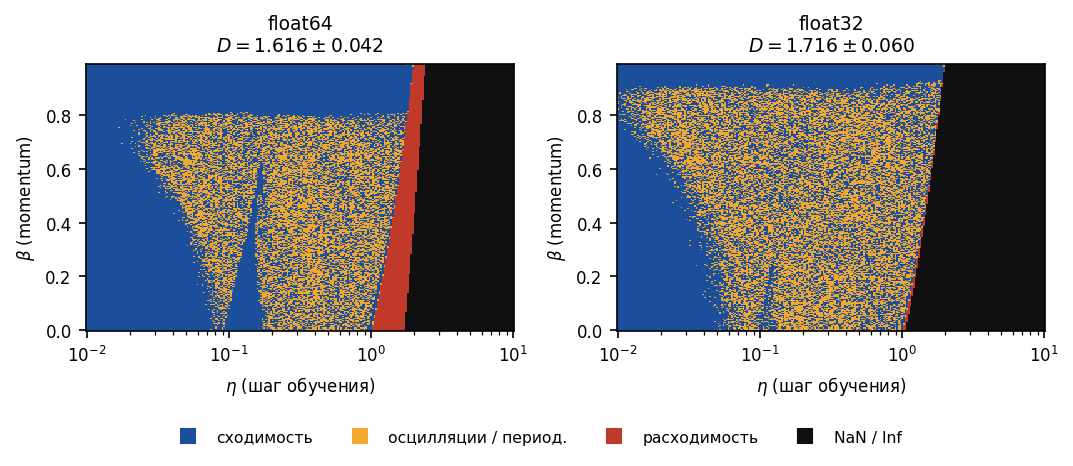
\includegraphics[width=\linewidth]{f15_precision.png}
  \caption{Одно и то же сечение $(\eta,\beta)$, вычисленное в двойной и
  одинарной точности.}
  \label{fig:prec}
\end{figure}

Крупномасштабная структура совпадает, что подтверждает: наблюдаемая
изрезанность не является артефактом численной ошибки. Оценка размерности в
одинарной точности оказалась выше ($\DFloatThirtyTwo$ против $\DWdZero$).
Это ожидаемо: в хаотической зоне траектории чувствительны к начальным
условиям, и ошибки округления в \texttt{float32} действуют как дополнительный
шум, увеличивая перемешивание режимов вблизи границы. Для измерения
размерности двойная точность необходима.

\section{Обсуждение}\label{sec:discussion}

\subsection{Сводка результатов}

Собранные данные позволяют дать следующие ответы на вопросы, поставленные
в разделе~\ref{sec:problem}.

\emph{Сохраняется ли фрактальность при добавлении инерции?} Да, полностью.
Размерность границы в сечении $(\eta,\beta)$ равна
$\DEtaBeta \pm \DEtaBetaS$ и совпадает в пределах погрешности с базовой картой
$(\eta_0,\eta_1)$, где $\DBaseTanh \pm \DBaseTanhS$. Инерция сдвигает границу,
меняет соотношение долей режимов, но не делает её гладкой.

\emph{Влияние затухания весов и размера батча.} Умеренное затухание весов
сглаживает границу; уменьшение размера батча, наоборот, увеличивает её
изрезанность монотонно ($\DMbFull \to \DMbFour \to \DMbOne$ при
$B = 32 \to 4 \to 1$). Оба эффекта естественно интерпретируются через
многомасштабность целевой функции: регуляризация подавляет мелкомасштабные
особенности ландшафта, стохастичность батча их добавляет.

\emph{Сглаживают ли адаптивные методы границу?} Ответ оказался тоньше, чем
предполагала исходная гипотеза, и составляет, на наш взгляд, основной
содержательный результат работы.

\subsection{О «сглаживании» границы адаптивными методами}

Гипотеза задания состояла в том, что адаптивные методы частично сглаживают
фрактальную структуру за счёт нормализации градиентов по координатам. Данные
подтверждают её в узком смысле и опровергают в широком.

В плоскости $(\eta_0,\eta_1)$ Adam действительно даёт меньшую размерность, чем
SGD ($\DAdam$ против $\DSgd$). Однако наименьшую размерность даёт не адаптивный
метод, а SGD с фиксированной инерцией $\beta=0.9$ ($\DMomentum$), где никакой
покоординатной нормализации нет. Значит, сглаживание обеспечивает не
адаптивность как таковая, а усреднение градиента по времени, которое подавляет
высокочастотную составляющую динамики и уменьшает чувствительность исхода
к малым изменениям шага.

Более того, сглаживание оказывается свойством выбранного \emph{сечения}, а не
оптимизатора. Стоит перерезать пространство гиперпараметров вдоль собственных
осей Adam, и граница вновь оказывается предельно изрезанной: $\DAdamBOne$ для
$(\eta,\beta_1)$ и $\DAdamBTwo$ для $(\eta,\beta_2)$ --- выше, чем у SGD в
базовом сечении. Механизм понятен из вида карт Adam и RMSprop
(рис.~\ref{fig:opt}): покоординатная нормализация делает величину шага по
каждому весу почти независимой от масштаба градиента, из-за чего динамика
разделяется по слоям и карта в плоскости $(\eta_0,\eta_1)$ становится почти
сепарабельной --- граница вырождается в набор почти горизонтальных полос.
Низкая размерность здесь измеряет сепарабельность, а не отсутствие хаоса.
Как только сечение выбирается так, что сепарабельность не работает
(оси $\beta_1$, $\beta_2$ управляют самим усреднением), фрактальность
проявляется в полной мере.

Этот вывод согласуется с результатами~\cite{torkamandi2025}, где фрактальные
границы наблюдались именно для моделей, обучаемых Adam, и
с~\cite{cohen2022}, где показано, что адаптивные методы обладают собственным
аналогом грани устойчивости. Практический смысл: переход на Adam не избавляет
от необходимости аккуратного подбора шага обучения, он лишь переносит
нерегулярность в другие координаты пространства гиперпараметров.

\subsection{Связь с теорией динамики}

Наблюдаемая картина хорошо укладывается в схему раздела~\ref{sec:theory}.
Для квадратичной модели граница устойчивости --- гладкая прямая
$\eta\lambda = 2(1+\beta)$. В карте $(\eta,\beta)$ (рис.~\ref{fig:etabeta})
внешняя граница области переполнения действительно близка к прямой линии,
смещающейся с ростом $\beta$; именно она соответствует линейной теории.
Вся нерегулярность сосредоточена на внутренней границе --- между сходимостью
и ограниченными колебаниями. Это в точности та зона, где линейный анализ
неприменим: система вышла за порог устойчивости по старшей моде, но не
расходится, потому что нелинейность переводит её в область меньшей
кривизны (catapult-механизм~\cite{lewkowycz2020}) или удерживает на грани
устойчивости~\cite{cohen2021}. Исход в этой зоне определяется тонким балансом
и потому чувствителен к сколь угодно малым изменениям гиперпараметров ---
что и порождает фрактальную структуру.

Бифуркационная диаграмма (рис.~\ref{fig:bif}) показывает механизм в чистом
виде: при росте $\eta$ нелинейная скалярная система проходит через каскад
удвоения периода и хаос, и рост $\beta$ смещает каскад в область меньших
шагов. Показательно, что для линейной задачи инерция допустимый шаг
расширяет (следствие 2), а для нелинейной --- сужает окно регулярного
поведения. Именно это расхождение между линейным предсказанием и нелинейной
реальностью и есть источник изрезанности границы.

\subsection{Ограничения исследования}\label{sec:limitations}

Результаты следует интерпретировать с учётом ряда существенных ограничений.

\textbf{Зависимость оценки размерности от разрешения сетки.} Это наиболее
серьёзное методологическое ограничение. Одна и та же конфигурация, посчитанная
на разных сетках, даёт систематически разные оценки (табл.~\ref{tab:res}):
от $\DResSmall$ на сетке $128\times128$ до $\DBaseTanh$ на $512\times512$.
Причина в том, что более мелкая сетка разрешает более тонкие складки границы,
а диапазон доступных масштабов $\varepsilon$ в формуле~\eqref{eq:box} всегда
ограничен снизу размером пикселя. Приводимая величина $\sigma_D$ отражает
только качество линейной регрессии и эту систематику не учитывает. Поэтому
сравнивать между собой корректно только карты одинакового разрешения, что
в настоящей работе и делается: все сравнения оптимизаторов, сечений и
датасетов выполнены на сетках $256\times256$.

\begin{table}[htbp]
  \centering
  \caption{Зависимость оценки размерности от разрешения сетки для одной и той
  же конфигурации (tanh, $(\eta_0,\eta_1)$, $|\mathcal{D}|=1$).}
  \label{tab:res}
  \small
  \input{tables/tab_resolution.tex}
\end{table}

\textbf{Различие окон сканирования.} Порог устойчивости зависит от активации,
объёма данных и оптимизатора, поэтому окна по $\eta$ подбирались
индивидуально. Как следствие, доля площади карты, занятая границей, различна
для разных экспериментов, а измеряемая размерность от неё зависит. Сравнение
размерностей между оптимизаторами является, строго говоря, качественным;
количественно надёжны лишь сравнения внутри одного семейства окон
(например, ряд по размеру батча, где окно фиксировано).

\textbf{Граница как зона, а не кривая.} В отличие от классических фракталов,
где граница --- одномерная кривая, в наших картах переход между сходимостью и
колебаниями представляет собой протяжённую зону, в которой режимы перемешаны
на масштабе отдельных узлов сетки. Значения $D\approx1.85$, полученные на
глубоких уровнях зума, отражают приближение этой зоны к площадному заполнению,
а не структуру гладкой кривой. Формально box-counting применим и здесь, но
интерпретировать результат как «размерность границы» следует с осторожностью.

\textbf{Артефакт критерия сходимости для ReLU.} Критерий, унаследованный от
предыдущей НИР (средний нормализованный loss меньше единицы), засчитывает как
успешное обучение вырожденный случай: при большом шаге все ReLU-нейроны
переходят в область отрицательных предактиваций, градиент обнуляется, обучение
останавливается, и loss замирает на постоянном уровне ниже начального. Мёртвая
сеть формально классифицируется как сошедшаяся. Именно этим объясняется доля
сходимости $0.99$ для ReLU при $|\mathcal{D}|=1$ во всём диапазоне вплоть до
$\eta = 10^{4}$. Для корректного сравнения активаций пришлось использовать
набор из 32 примеров, где такой коллапс менее вероятен. Более строгий критерий
(требование снижения loss в заданное число раз) устранил бы артефакт, но
сделал бы результаты несопоставимыми с предыдущей работой.

\textbf{Ограниченность числа итераций.} Все эксперименты выполнены при
$T = 400$. Классификация режимов зависит от $T$: траектория, помеченная как
осциллирующая, могла бы при большем $T$ выйти на сходимость. Это смещает
границу в сторону области колебаний, но, судя по устойчивости картины при
переходе от $T=300$ к $T=500$ на этапе калибровки, не меняет качественных
выводов.

\textbf{Простота архитектуры и объём данных.} Исследована однослойная сеть с
512 параметрами на выборках объёмом до 32 примеров. Перенос выводов на
глубокие архитектуры и полноразмерные датасеты требует отдельной проверки;
косвенным аргументом в пользу переносимости служит работа~\cite{torkamandi2025},
где явление наблюдалось для трансформеров.

\textbf{Отсутствие прямого трёхмерного box-counting.} Трёхмерное пространство
исследовано набором двумерных сечений; как показано в разделе~\ref{sec:3d},
немонотонность $D(\lambda_{wd})$ не позволяет по сечениям надёжно судить о
размерности трёхмерной границы.

\subsection{Практические следствия}

Из полученных данных вытекает несколько практических соображений.
Во-первых, автоматический подбор шага обучения принципиально осложнён тем, что
на любом масштабе рядом с работающей конфигурацией находится неработающая;
это относится и к SGD, и к Adam, только для последнего нерегулярность
проявляется в других координатах. Во-вторых, наилучшие по скорости
конфигурации систематически лежат вблизи границы, что согласуется с концепцией
грани устойчивости и означает, что консервативный выбор шага заведомо жертвует
скоростью. В-третьих, умеренная $L_2$-регуляризация и увеличение размера батча
делают ландшафт обучаемости более предсказуемым --- это может быть
самостоятельным аргументом в их пользу помимо влияния на обобщающую
способность.

\section{Заключение}\label{sec:conclusion}

\subsection{Достигнутые результаты}

В работе исследована структура границы обучаемости однослойной нейронной сети
в многомерном пространстве гиперпараметров, включающем шаг обучения, инерцию,
затухание весов, размер мини-батча и параметры адаптивных оптимизаторов.
Получены следующие результаты.

\begin{enumerate}[leftmargin=*,topsep=2pt,itemsep=3pt]
  \item \textbf{Теоретический мини-результат.} Для квадратичной функции
        $L(w)=\tfrac12\lambda w^2$ градиентный спуск с инерцией записан в виде
        двумерного линейного отображения с матрицей перехода
        $M = \bigl(\begin{smallmatrix} 1-\eta\lambda & -\eta\beta \\ \lambda & \beta \end{smallmatrix}\bigr)$,
        для которой $\det M = \beta$ и $\operatorname{tr} M = 1+\beta-\eta\lambda$.
        Доказано (предложение~\ref{prop:stab}), что область устойчивости есть
        $0 < \eta\lambda < 2(1+\beta)$ при $|\beta|<1$, то есть инерция
        расширяет допустимый шаг обучения вплоть до двукратного по сравнению
        с обычным градиентным спуском; при комплексных собственных значениях
        скорость сходимости равна $\sqrt{\beta}$ и не зависит от кривизны.
        Результат подтверждён численно.
  \item \textbf{Репликация.} Воспроизведён базовый эксперимент предыдущей НИР;
        для активации tanh на сетке $512\times512$ получено
        $D_{\mathrm{box}} = \DBaseTanh \pm \DBaseTanhS$. Показано, что
        сравнение активаций требует индивидуального выбора окна сканирования,
        поскольку порог устойчивости у них различается на порядки.
  \item \textbf{Фрактальность сохраняется при добавлении инерции.} В сечении
        $(\eta,\beta)$ получено $D_{\mathrm{box}} = \DEtaBeta \pm \DEtaBetaS$,
        что совпадает с базовой картой в пределах погрешности.
  \item \textbf{Влияние регуляризации и батча.} Затухание весов сглаживает
        границу ($\DEtaWd$ против $\DSgd$ при том же разрешении), уменьшение
        размера батча --- увеличивает изрезанность монотонно:
        $\DMbFull$, $\DMbFour$, $\DMbOne$ при $B=32,4,1$.
  \item \textbf{Сравнение оптимизаторов.} Получены размерности $\DSgd$ (SGD),
        $\DMomentum$ (SGD с инерцией $\beta=0.9$), $\DAdam$ (Adam),
        $\DRmsprop$ (RMSprop). Гипотеза о сглаживающем действии адаптивных
        методов подтверждается лишь частично: сглаживание обеспечивает
        усреднение градиента по времени, а не покоординатная нормализация, и
        является свойством выбранного сечения --- в сечениях $(\eta,\beta_1)$
        и $(\eta,\beta_2)$ сам Adam даёт $\DAdamBOne$ и $\DAdamBTwo$.
  \item \textbf{Структурированные данные.} Переход от случайных данных к набору
        digits увеличивает размерность границы ($\DSynth \to \DDigits$);
        фрактальность не является артефактом синтетических данных.
  \item \textbf{Трёхмерное пространство.} Построены четыре сечения
        $(\eta,\beta)$ при разных $\lambda_{wd}$; зависимость размерности от
        $\lambda_{wd}$ немонотонна, что показывает ограниченность вывода о
        трёхмерной границе по набору двумерных сечений.
  \item \textbf{Воспроизводимый инструментарий.} Реализована ансамблевая
        векторизованная схема сканирования, позволяющая обсчитывать сетки
        $512\times512$ на одном ядре CPU за единицы минут, с фиксацией seed,
        точности и полным сохранением параметров каждого запуска.
\end{enumerate}

\subsection{Научная и практическая значимость}

Основной содержательный вывод состоит в том, что фрактальность границы
обучаемости --- свойство не конкретного оптимизатора, а самой нелинейной
динамики обучения вблизи порога устойчивости. Переход к более сложным
оптимизаторам меняет расположение границы и то, в каких координатах
проявляется её нерегулярность, но не устраняет её. Это уточняет ожидание,
согласно которому адаптивные методы «сглаживают» ландшафт обучаемости.

Практически это означает, что чувствительность к шагу обучения не может быть
устранена выбором оптимизатора и должна учитываться в процедурах
автоматического подбора гиперпараметров; при этом умеренная $L_2$-регуляризация
и увеличение размера батча объективно повышают предсказуемость обучения.

\subsection{Ограничения}

Основные ограничения перечислены в разделе~\ref{sec:limitations}. Кратко:
оценка размерности систематически зависит от разрешения сетки, что допускает
сравнение лишь внутри одного разрешения; окна сканирования подбирались
индивидуально, что делает межоптимизаторное сравнение качественным; переход
между режимами представляет собой протяжённую зону перемешивания, а не
кривую; критерий сходимости, унаследованный от предыдущей работы, засчитывает
как успех вырожденный случай «мёртвых» ReLU-нейронов; исследована лишь
однослойная сеть при $T=400$ итерациях.

\subsection{Направления дальнейшей работы}

\begin{enumerate}[leftmargin=*,topsep=2pt,itemsep=2pt]
  \item Прямой трёхмерный box-counting в пространстве
        $(\eta,\beta,\lambda_{wd})$ вместо набора сечений; это требует
        примерно двух порядков дополнительного машинного времени либо
        адаптивного разрешения сетки вблизи границы.
  \item Уточнение критерия обучаемости: замена порога «loss ниже начального»
        на требование снижения loss в заданное число раз с отдельной
        классификацией вырожденных состояний (мёртвые нейроны, стягивание
        весов к нулю регуляризацией).
  \item Проверка устойчивости выводов к числу итераций: измерение
        $D_{\mathrm{box}}(T)$ и определение, сходится ли оценка при $T\to\infty$.
  \item Перенос сравнения оптимизаторов на глубокие архитектуры и на
        полноразмерные датасеты, включая проверку сепарабельности карт Adam,
        обнаруженной в настоящей работе.
  \item Развязанное затухание весов (AdamW)~\cite{loshchilov2019} как отдельное
        сечение: интересно, сохраняется ли сглаживающий эффект при развязке.
  \item Аналитическое описание внутренней границы (между сходимостью и
        ограниченными колебаниями) для двухслойной линейной сети, где
        динамика допускает явный анализ.
\end{enumerate}


\newpage
\begin{thebibliography}{99}
\addcontentsline{toc}{section}{Список литературы}

\bibitem{sohl2024}
\emph{Sohl-Dickstein J.} The boundary of neural network trainability is fractal
// arXiv preprint arXiv:2402.06184. --- 2024. --- URL:
\url{https://arxiv.org/abs/2402.06184} (дата обращения: 20.05.2026).

\bibitem{torkamandi2025}
\emph{Torkamandi B. [и др.]} Mapping the edge of chaos: fractal-like boundaries
in the trainability of decoder-only transformer models // arXiv preprint
arXiv:2501.04286. --- 2025. --- URL: \url{https://arxiv.org/abs/2501.04286}
(дата обращения: 20.05.2026).

\bibitem{liu2024}
\emph{Liu Y., Arnould L., Sohl-Dickstein J.} Complex fractal trainability
boundary can arise from trivial non-convexity // arXiv preprint
arXiv:2406.13971. --- 2024. --- URL: \url{https://arxiv.org/abs/2406.13971}
(дата обращения: 20.05.2026).

\bibitem{cohen2021}
\emph{Cohen J. M., Kaur S., Li Y., Kolter J. Z., Talwalkar A.} Gradient descent
on neural networks typically occurs at the edge of stability //
International Conference on Learning Representations (ICLR). --- 2021. --- URL:
\url{https://arxiv.org/abs/2103.00065} (дата обращения: 20.05.2026).

\bibitem{cohen2022}
\emph{Cohen J. M. [и др.]} Adaptive gradient methods at the edge of stability
// arXiv preprint arXiv:2207.14484. --- 2022. --- URL:
\url{https://arxiv.org/abs/2207.14484} (дата обращения: 20.05.2026).

\bibitem{lewkowycz2020}
\emph{Lewkowycz A., Bahri Y., Dyer E., Sohl-Dickstein J., Gur-Ari G.} The large
learning rate phase of deep learning: the catapult mechanism // arXiv preprint
arXiv:2003.02218. --- 2020. --- URL: \url{https://arxiv.org/abs/2003.02218}
(дата обращения: 20.05.2026).

\bibitem{kong2020}
\emph{Kong L., Tao M.} Stochasticity of deterministic gradient descent: large
learning rate for multiscale objective function // Advances in Neural
Information Processing Systems (NeurIPS). --- 2020. --- URL:
\url{https://proceedings.neurips.cc/paper/2020/file/1b9a80606d74d3da6db2f1274557e644-Paper.pdf}
(дата обращения: 20.05.2026).

\bibitem{chen2023}
\emph{Chen X., Balasubramanian K., Ghosal P., Agrawalla B.} From stability to
chaos: analyzing gradient descent dynamics in quadratic regression //
arXiv preprint arXiv:2310.01687. --- 2023. --- URL:
\url{https://arxiv.org/abs/2310.01687} (дата обращения: 20.05.2026).

\bibitem{feigenbaum1978}
\emph{Feigenbaum M. J.} Quantitative universality for a class of nonlinear
transformations // Journal of Statistical Physics. --- 1978. --- Т. 19,
№ 1. --- С. 25--52. --- DOI: 10.1007/BF01020332.

\bibitem{liyorke1975}
\emph{Li T.-Y., Yorke J. A.} Period three implies chaos // The American
Mathematical Monthly. --- 1975. --- Т. 82, № 10. --- С. 985--992. ---
DOI: 10.2307/2318254.

\bibitem{polyak1964}
\emph{Поляк Б. Т.} О некоторых способах ускорения сходимости итерационных
методов // Журнал вычислительной математики и математической физики. ---
1964. --- Т. 4, № 5. --- С. 791--803.

\bibitem{nesterov1983}
\emph{Нестеров Ю. Е.} Метод решения задачи выпуклого программирования со
скоростью сходимости $O(1/k^2)$ // Доклады АН СССР. --- 1983. --- Т. 269,
№ 3. --- С. 543--547.

\bibitem{kingma2015}
\emph{Kingma D. P., Ba J.} Adam: a method for stochastic optimization //
International Conference on Learning Representations (ICLR). --- 2015. --- URL:
\url{https://arxiv.org/abs/1412.6980} (дата обращения: 20.05.2026).

\bibitem{tieleman2012}
\emph{Tieleman T., Hinton G.} Lecture 6.5---RMSprop: divide the gradient by a
running average of its recent magnitude // COURSERA: Neural Networks for
Machine Learning. --- 2012.

\bibitem{loshchilov2019}
\emph{Loshchilov I., Hutter F.} Decoupled weight decay regularization //
International Conference on Learning Representations (ICLR). --- 2019. --- URL:
\url{https://arxiv.org/abs/1711.05101} (дата обращения: 20.05.2026).

\bibitem{bottou2018}
\emph{Bottou L., Curtis F. E., Nocedal J.} Optimization methods for large-scale
machine learning // SIAM Review. --- 2018. --- Т. 60, № 2. --- С. 223--311. ---
DOI: 10.1137/16M1080173.

\bibitem{smith2018}
\emph{Smith S. L., Kindermans P.-J., Ying C., Le Q. V.} Don't decay the learning
rate, increase the batch size // International Conference on Learning
Representations (ICLR). --- 2018. --- URL:
\url{https://arxiv.org/abs/1711.00489} (дата обращения: 20.05.2026).

\bibitem{goodfellow2016}
\emph{Goodfellow I., Bengio Y., Courville A.} Deep Learning. --- Cambridge, MA:
MIT Press, 2016. --- 800 с. --- URL: \url{http://www.deeplearningbook.org}
(дата обращения: 20.05.2026).

\bibitem{falconer2014}
\emph{Falconer K.} Fractal Geometry: Mathematical Foundations and
Applications. --- 3rd ed. --- Chichester: Wiley, 2014. --- 400 с.

\bibitem{mandelbrot1982}
\emph{Mandelbrot B. B.} The Fractal Geometry of Nature. --- New York:
W. H. Freeman and Company, 1982. --- 468 с.

\bibitem{strogatz2015}
\emph{Strogatz S. H.} Nonlinear Dynamics and Chaos: With Applications to
Physics, Biology, Chemistry, and Engineering. --- 2nd ed. --- Boulder, CO:
Westview Press, 2015. --- 513 с.

\bibitem{porespy2019}
\emph{Gostick J. T. [и др.]} PoreSpy: a Python toolkit for quantitative
analysis of porous media images // Journal of Open Source Software. ---
2019. --- Т. 4, № 37. --- С. 1296. --- URL:
\url{https://porespy.org/examples/metrics/tutorials/computing_fractal_dim.html}
(дата обращения: 20.05.2026).

\bibitem{harris2020}
\emph{Harris C. R. [и др.]} Array programming with NumPy // Nature. ---
2020. --- Т. 585. --- С. 357--362. --- DOI: 10.1038/s41586-020-2649-2.

\bibitem{virtanen2020}
\emph{Virtanen P. [и др.]} SciPy 1.0: fundamental algorithms for scientific
computing in Python // Nature Methods. --- 2020. --- Т. 17. --- С. 261--272. ---
DOI: 10.1038/s41592-019-0686-2.

\bibitem{pedregosa2011}
\emph{Pedregosa F. [и др.]} Scikit-learn: machine learning in Python //
Journal of Machine Learning Research. --- 2011. --- Т. 12. --- С. 2825--2830.

\bibitem{skimage2014}
\emph{van der Walt S. [и др.]} scikit-image: image processing in Python //
PeerJ. --- 2014. --- Т. 2. --- С. e453. --- DOI: 10.7717/peerj.453.

\end{thebibliography}


\newpage
\appendix
\section{Исходный код}\label{app:code}

Полный исходный код, конфигурации и сохранённые результаты доступны в
репозитории проекта:
\begin{center}
\url{https://github.com/obilka/fractal_hyperparams_project}
\end{center}
Структура каталогов описана в приложении~\ref{app:repro}.
Ниже приведены ключевые фрагменты.

\subsection{Ансамблевая итерация обучения}

Основной приём реализации --- одновременное обучение всех узлов сетки
гиперпараметров как ансамбля независимых сетей. Веса хранятся с ведущей осью
$G$ (номер конфигурации), гиперпараметры транслируются по осям весов.

\begin{lstlisting}[language=Python,caption={Прямой и обратный проход для ансамбля сетей}]
H  = np.einsum("nd,ghd->gnh", Xb, W0, optimize=True)
Ha = _act(H, cfg.activation)
out = np.einsum("gnh,goh->gno", Ha, W1, optimize=True)
R = out - Yb
loss = np.einsum("gno,gno->g", R, R) / (Nb * d_out)

# ручное обратное распространение
go  = (2.0 / (Nb * d_out)) * R
gW1 = np.einsum("gno,gnh->goh", go, Ha, optimize=True)
gha = np.einsum("gno,goh->gnh", go, W1, optimize=True)
gh  = gha * _act_grad(H, Ha, cfg.activation)
gW0 = np.einsum("gnh,nd->ghd", gh, Xb, optimize=True)

# L2-регуляризация (weight decay)
gW0 = gW0 + wd * W0
gW1 = gW1 + wd * W1
\end{lstlisting}

\subsection{Правила обновления}

\begin{lstlisting}[language=Python,caption={Реализация четырёх оптимизаторов}]
if opt == "sgd":
    W0 -= lr0 * gW0
    W1 -= lr1 * gW1
elif opt == "momentum":
    M0 = beta * M0 + gW0
    M1 = beta * M1 + gW1
    W0 -= lr0 * M0
    W1 -= lr1 * M1
elif opt == "rmsprop":
    V0 = b2 * V0 + (1 - b2) * gW0 * gW0
    V1 = b2 * V1 + (1 - b2) * gW1 * gW1
    W0 -= lr0 * gW0 / (np.sqrt(V0) + eps)
    W1 -= lr1 * gW1 / (np.sqrt(V1) + eps)
elif opt == "adam":
    M0 = b1 * M0 + (1 - b1) * gW0
    V0 = b2 * V0 + (1 - b2) * gW0 * gW0
    bc1, bc2 = 1 - np.power(b1, t + 1), 1 - np.power(b2, t + 1)
    W0 -= lr0 * (M0 / bc1) / (np.sqrt(V0 / bc2) + eps)
    # аналогично для второго слоя
\end{lstlisting}

\subsection{Классификация режимов}

\begin{lstlisting}[language=Python,caption={Классификация траектории на четыре режима}]
m20       = tail[:, -TAIL_SHORT:].mean(axis=1)
m20_first = tail[:, :TAIL_SHORT].mean(axis=1)
rel       = tail.std(axis=1) / np.maximum(tail.mean(axis=1), 1e-300)

stabilized = rel < CONV_TOL              # вышли на стационар
decreasing = m20 < 0.99 * m20_first      # loss продолжает убывать
conv = (m20 < 1.0) & (stabilized | decreasing) & np.isfinite(m20)
div  = (stats["max_l"] > DIV_THRESHOLD) | (m20 > DIV_THRESHOLD)

regime[:]             = OSCILLATING
regime[conv]          = CONVERGED
regime[div & ~nonfin] = DIVERGED
regime[nonfin]        = NONFINITE
\end{lstlisting}

\subsection{Извлечение границы и box-counting}

\begin{lstlisting}[language=Python,caption={Морфологическое извлечение границы и оценка размерности}]
def extract_boundary(regime):
    B = (regime == CONVERGED)
    st = ndimage.generate_binary_structure(2, 1)
    bnd = np.logical_xor(ndimage.binary_dilation(B, structure=st),
                         ndimage.binary_erosion(B, structure=st))
    return skeletonize(bnd) if bnd.sum() > 0 else bnd

def box_counting_dimension(boundary, min_box=2, max_div=8):
    s, sizes, counts = min_box, [], []
    while s <= max(min_box * 2, min(boundary.shape) // max_div):
        ny = (boundary.shape[0] // s) * s
        nx = (boundary.shape[1] // s) * s
        red = boundary[:ny, :nx].reshape(ny // s, s, nx // s, s).any(axis=(1, 3))
        if red.sum() > 0:
            sizes.append(s); counts.append(int(red.sum()))
        s *= 2
    coef, cov = np.polyfit(np.log(sizes), np.log(counts), 1, cov=True)
    return -coef[0], float(np.sqrt(cov[0, 0])), sizes, counts
\end{lstlisting}

\subsection{Теоретический блок}

\begin{lstlisting}[language=Python,caption={Спектральный радиус матрицы перехода метода с инерцией}]
def momentum_spectral_radius(eta_lambda, beta):
    x, b = np.asarray(eta_lambda), np.asarray(beta)
    tr, det = 1.0 + b - x, b
    disc = tr * tr - 4.0 * det
    sq = np.sqrt(np.abs(disc))
    r_real = np.maximum(np.abs((tr + sq) / 2.0), np.abs((tr - sq) / 2.0))
    return np.where(disc >= 0, r_real, np.sqrt(np.abs(det)))
\end{lstlisting}

\section{Инструкция по воспроизведению}\label{app:repro}

\subsection{Структура проекта}

\begin{verbatim}
src/fractal_hp.py        ядро: модель, оптимизаторы, сканирование,
                         box-counting, теоретический блок
src/run_experiments.py   все эксперименты (стадии A-H), resume-режим
src/make_figures.py      построение всех рисунков
src/make_tables.py       генерация LaTeX-таблиц и макросов с числами
report/main.tex          отчёт (XeLaTeX)
report/sections/         разделы отчёта
report/tables/           таблицы, генерируются автоматически
report/figures/          подпись для титульного листа
outputs/data/            результаты сканирований (.npz) и метаданные (.json)
outputs/figures/         рисунки
run_all.sh               полный цикл: расчёты, рисунки, таблицы, сборка PDF
requirements.txt         версии библиотек
\end{verbatim}

\subsection{Требования}

Python 3.10 и выше; NumPy, SciPy, scikit-image, scikit-learn, Matplotlib.
PyTorch не требуется. Для сборки отчёта --- \TeX{}Live с XeLaTeX и пакетами
polyglossia, fontspec, geometry, setspace, booktabs, subcaption, listings,
hyperref; шрифт Liberation Serif. Оперативной памяти достаточно 2 ГБ,
расчёты выполняются на CPU.

\subsection{Запуск}

\begin{lstlisting}[language=bash,caption={Полный цикл воспроизведения}]
git clone https://github.com/obilka/fractal_hyperparams_project.git
cd fractal_hyperparams_project
pip install -r requirements.txt
bash run_all.sh
\end{lstlisting}

Скрипт последовательно выполняет расчёты (стадии A--H), строит рисунки и
таблицы и собирает PDF. Отдельные стадии запускаются как
\texttt{python3 src/run\_experiments.py B C}. Расчёт поддерживает
возобновление: результат каждого блока из 4096 конфигураций сохраняется в
файл контрольной точки, и повторный запуск продолжает работу с места
остановки, а уже завершённые эксперименты пропускаются.

Суммарное машинное время всех экспериментов --- \TotalHours~ч на одном ядре
CPU.

\subsection{Фиксация случайности и точности}

Seed равен 42 для генерации данных, $42+1000$ для инициализации весов и
$42+7$ для порядка примеров в мини-батчах. Инициализация одинакова для всех
узлов сетки в пределах одного эксперимента. Тип данных по умолчанию
\texttt{float64}; эксперимент G1 выполнен в \texttt{float32} для оценки
влияния точности. Все параметры запуска сохраняются в JSON рядом с
результатом.

\section{Дополнительные материалы}

Числовые значения, приведённые в тексте и таблицах отчёта, подставляются
автоматически из файлов \texttt{outputs/data/*.json} через генерируемый файл
\texttt{report/tables/numbers.tex}. Это гарантирует, что текст отчёта,
таблицы и сохранённые результаты расчётов не могут разойтись между собой:
при повторном запуске расчётов и пересборке отчёта все числа обновляются
согласованно.


\end{document}
